\subsection{Network Configuration}
\label{subsec:network-config}
As touched on when discussing netplan (section \ref{sec:netplan.yml}) \parencite{Ubuntu2024NetplanDesign} the 3 NICs must be configured with the correct IP addressing scheme and networks. Figure \ref{fig:basic-fw-breakdown} shows a high-level breakdown of the firewall zones and NICs, each for a different usecase and level of security. This config is deployed via Ansible for consistency and to adhere to the DevOps practices mentioned in section \ref{sec:IaC}. The networks should be manually assigned to allow for some level of persistence, the firewall as the gateway for each internal zone:

\begin{table}[H]
\centering
\begin{tabular}{|l|l|l|l|}
\hline
\textbf{Zone} & \textbf{Interface} & \textbf{Network} & \textbf{Firewall IP} \\ \hline
WAN (Internet) & eth0 & 10.0.0.0/8 & 10.0.0.5/8 \\ \hline
LAN (Trusted) & eth1 & 172.16.0.0/16 & 172.16.0.1/16 \\ \hline
Guest (IoT) & eth2 & 192.168.0.0/24 & 192.168.0.1/24 \\ \hline
\end{tabular}
\caption{IP addressing for each firewall zone}
\label{tab:ip-addressing}
\end{table}

The netplan role structure follows Ansible best practices:

\begin{verbatim}
roles/netplan/
├── tasks/main.yml          # Deployment tasks
├── templates/netplan.j2     # Jinja2 netplan template
├── vars/main.yml           # Network configuration variables
└── handlers/main.yml       # Netplan apply handler
\end{verbatim}

Figure \ref{fig:netplan-tasks} shows the Ansible task list that disables Ubuntu's cloud-init network management (which conflicts with static configuration) and deploys the templated netplan configuration file.

\begin{figure}[H]
    \centering
    \begin{minted}{YAML}
    Hello
    \end{minted}
    \caption{The playbook used to deploy the Iptables config to the test (and production) firewall}
    \label{code:ansible-neplan-tasks}
\end{figure}

The first task creates a new cloud-init file that stops Ubuntu from creating / using it's own network configuration and preventing cloud-init from reverting back on subsequent boots. The second task deploys the Jinja2-templated netplan configuration to \texttt{/etc/netplan/50-cloud-init.yaml}, creating a backup of any existing configuration before overwriting.

\begin{figure}[H]
    \centering
    \begin{minted}{YAML}
    Hey there
    \end{minted}
    \caption{The handlers used for the netplan role}
    \label{code:ansible-neplan-handlers}
\end{figure}

Both tasks trigger the \texttt{netplan apply} handler (Figure \ref{code:ansible-neplan-handlers}), which applies the new netplan config without needing a system reboot.


\subsubsection{Installing NIC drivers}
The coursework provides an additional NIC so this firewall is able to accommodate all 3 zones at the same time. To determine the type of NIC I was given I checked the connected usb devices and picked the appropriate entry provided in the VLE (figure \ref{fig:command-lsusb} and driver \parencite{Morrownr2024_8812au_Driver})

\begin{figure}[H]
    \centering
    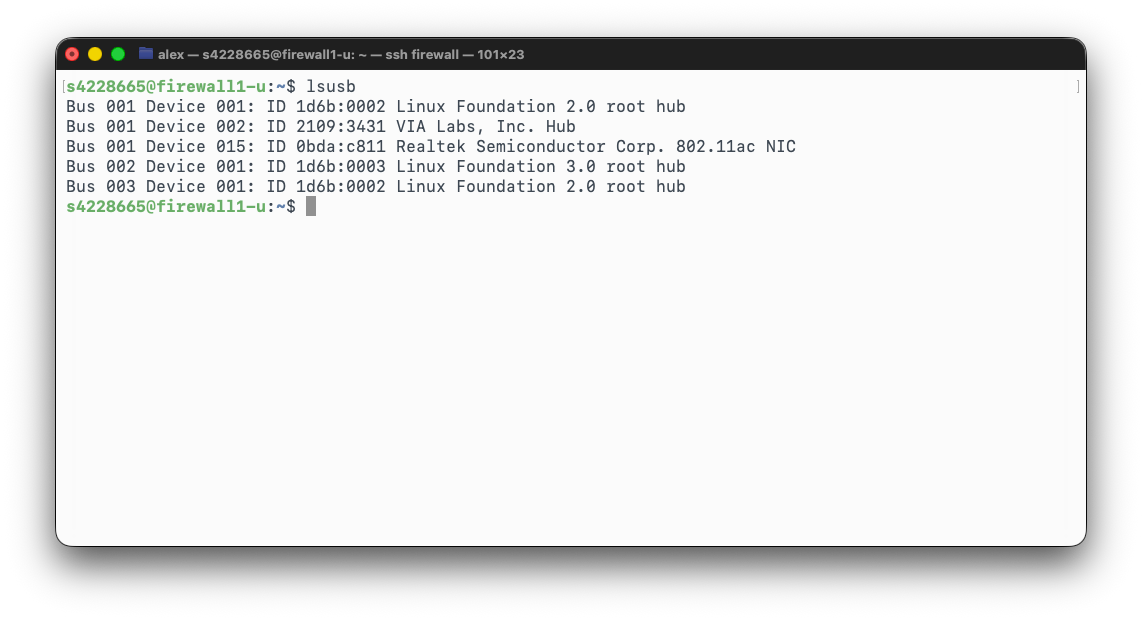
\includegraphics[width=0.8\linewidth]{Screenshots/command-lsusb.png}
    \caption{Enter Caption}
    \label{fig:command-lsusb}
\end{figure}

To install the driver I followed the steps from the repo \parencite{Morrownr2024_8812au_Driver} and collapsed them into a playbook called \verb|provision.yml| \ref{code:ansible-provision-playbook}. This playbook provisions both the test environment and the production firewall, only running certain plays on certain hosts (e.g. my user will already be on the Pi but not a newly made test environment).

\begin{figure}[H]
    \centering
    \begin{minted}{YAML}
    I'm the strongest dude
    \end{minted}
    \caption{The handlers used for the netplan role}
    \label{code:ansible-provision-playbook}
\end{figure}

We can test this by running the playbook via vagrant using \verb|vagrant up| when the playbook is referenced in the \verb|vagrantfile|, the output for this can be seen in figure \ref{vagrant:provision-vm-nic}.

\begin{figure}[H]
    \centering
    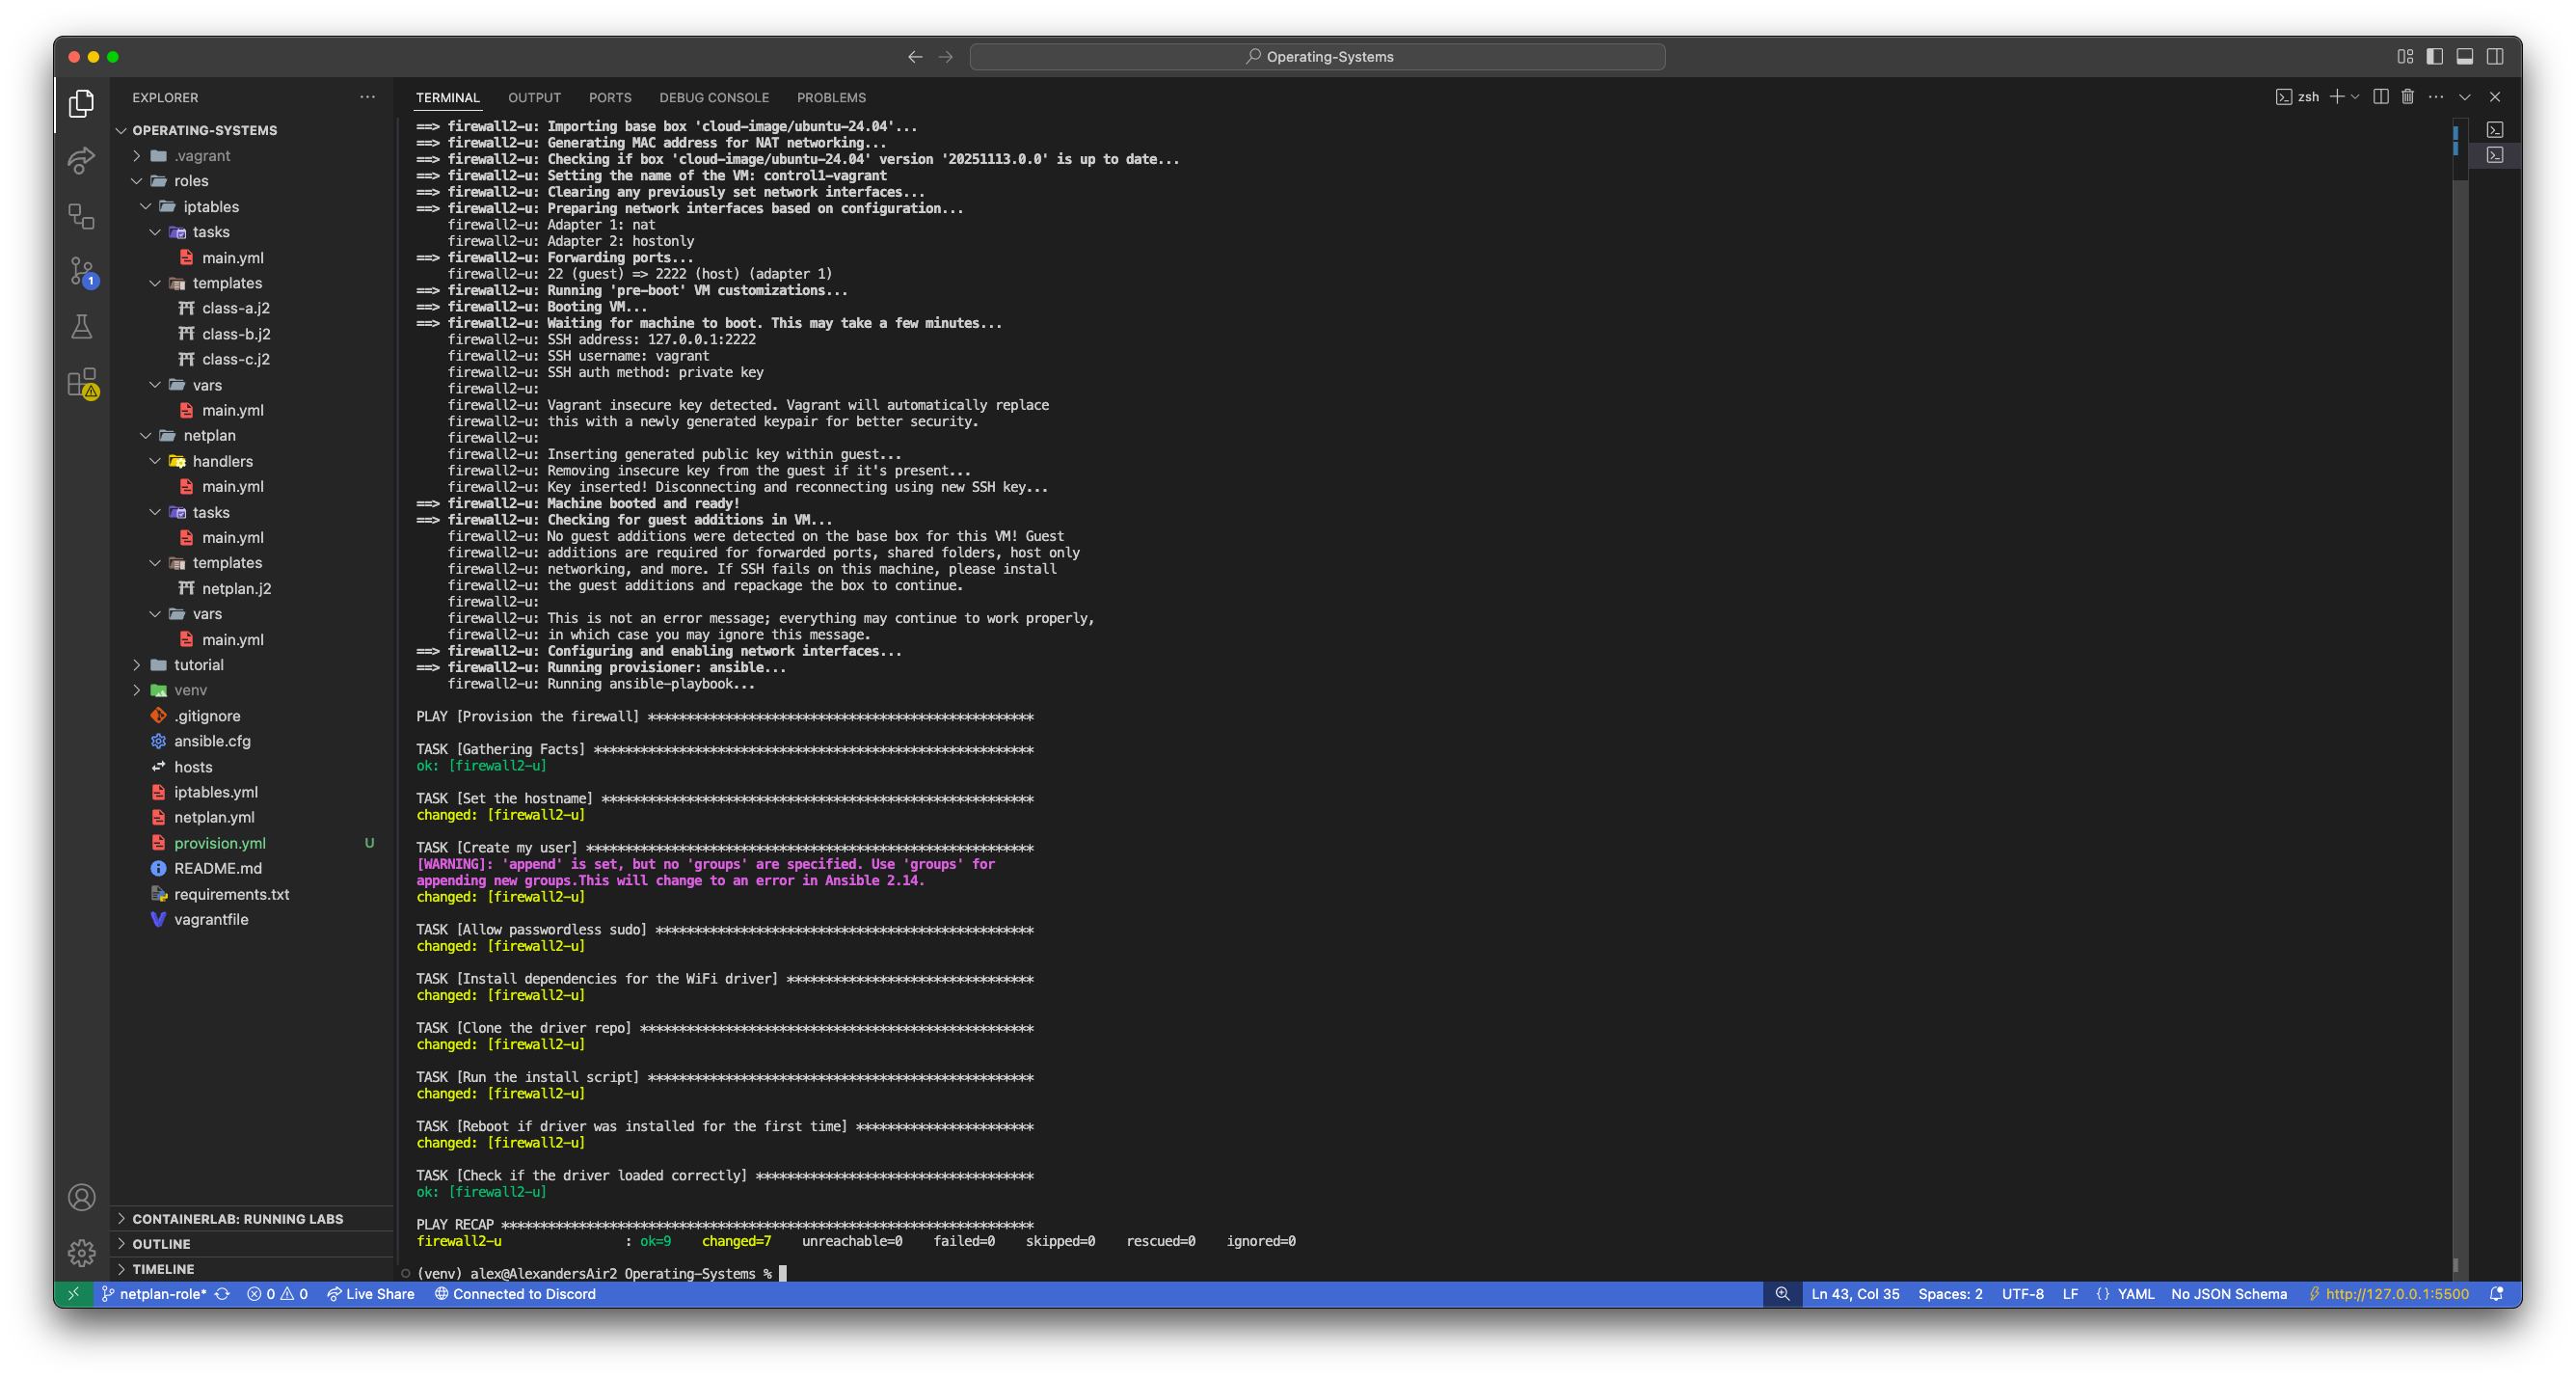
\includegraphics[width=\linewidth]{Screenshots/vscode-vagrant-provision.png}
    \caption{The output from bringing the provisioned VM with the driver up}
    \label{vagrant:provision-vm-nic}
\end{figure}

As the install was successful on the VM, it can be run on the production environment (Pi) and validated with \verb|| (figure \ref{vagrant:provision-firewall-nic}).

\begin{figure}[H]
    \centering
    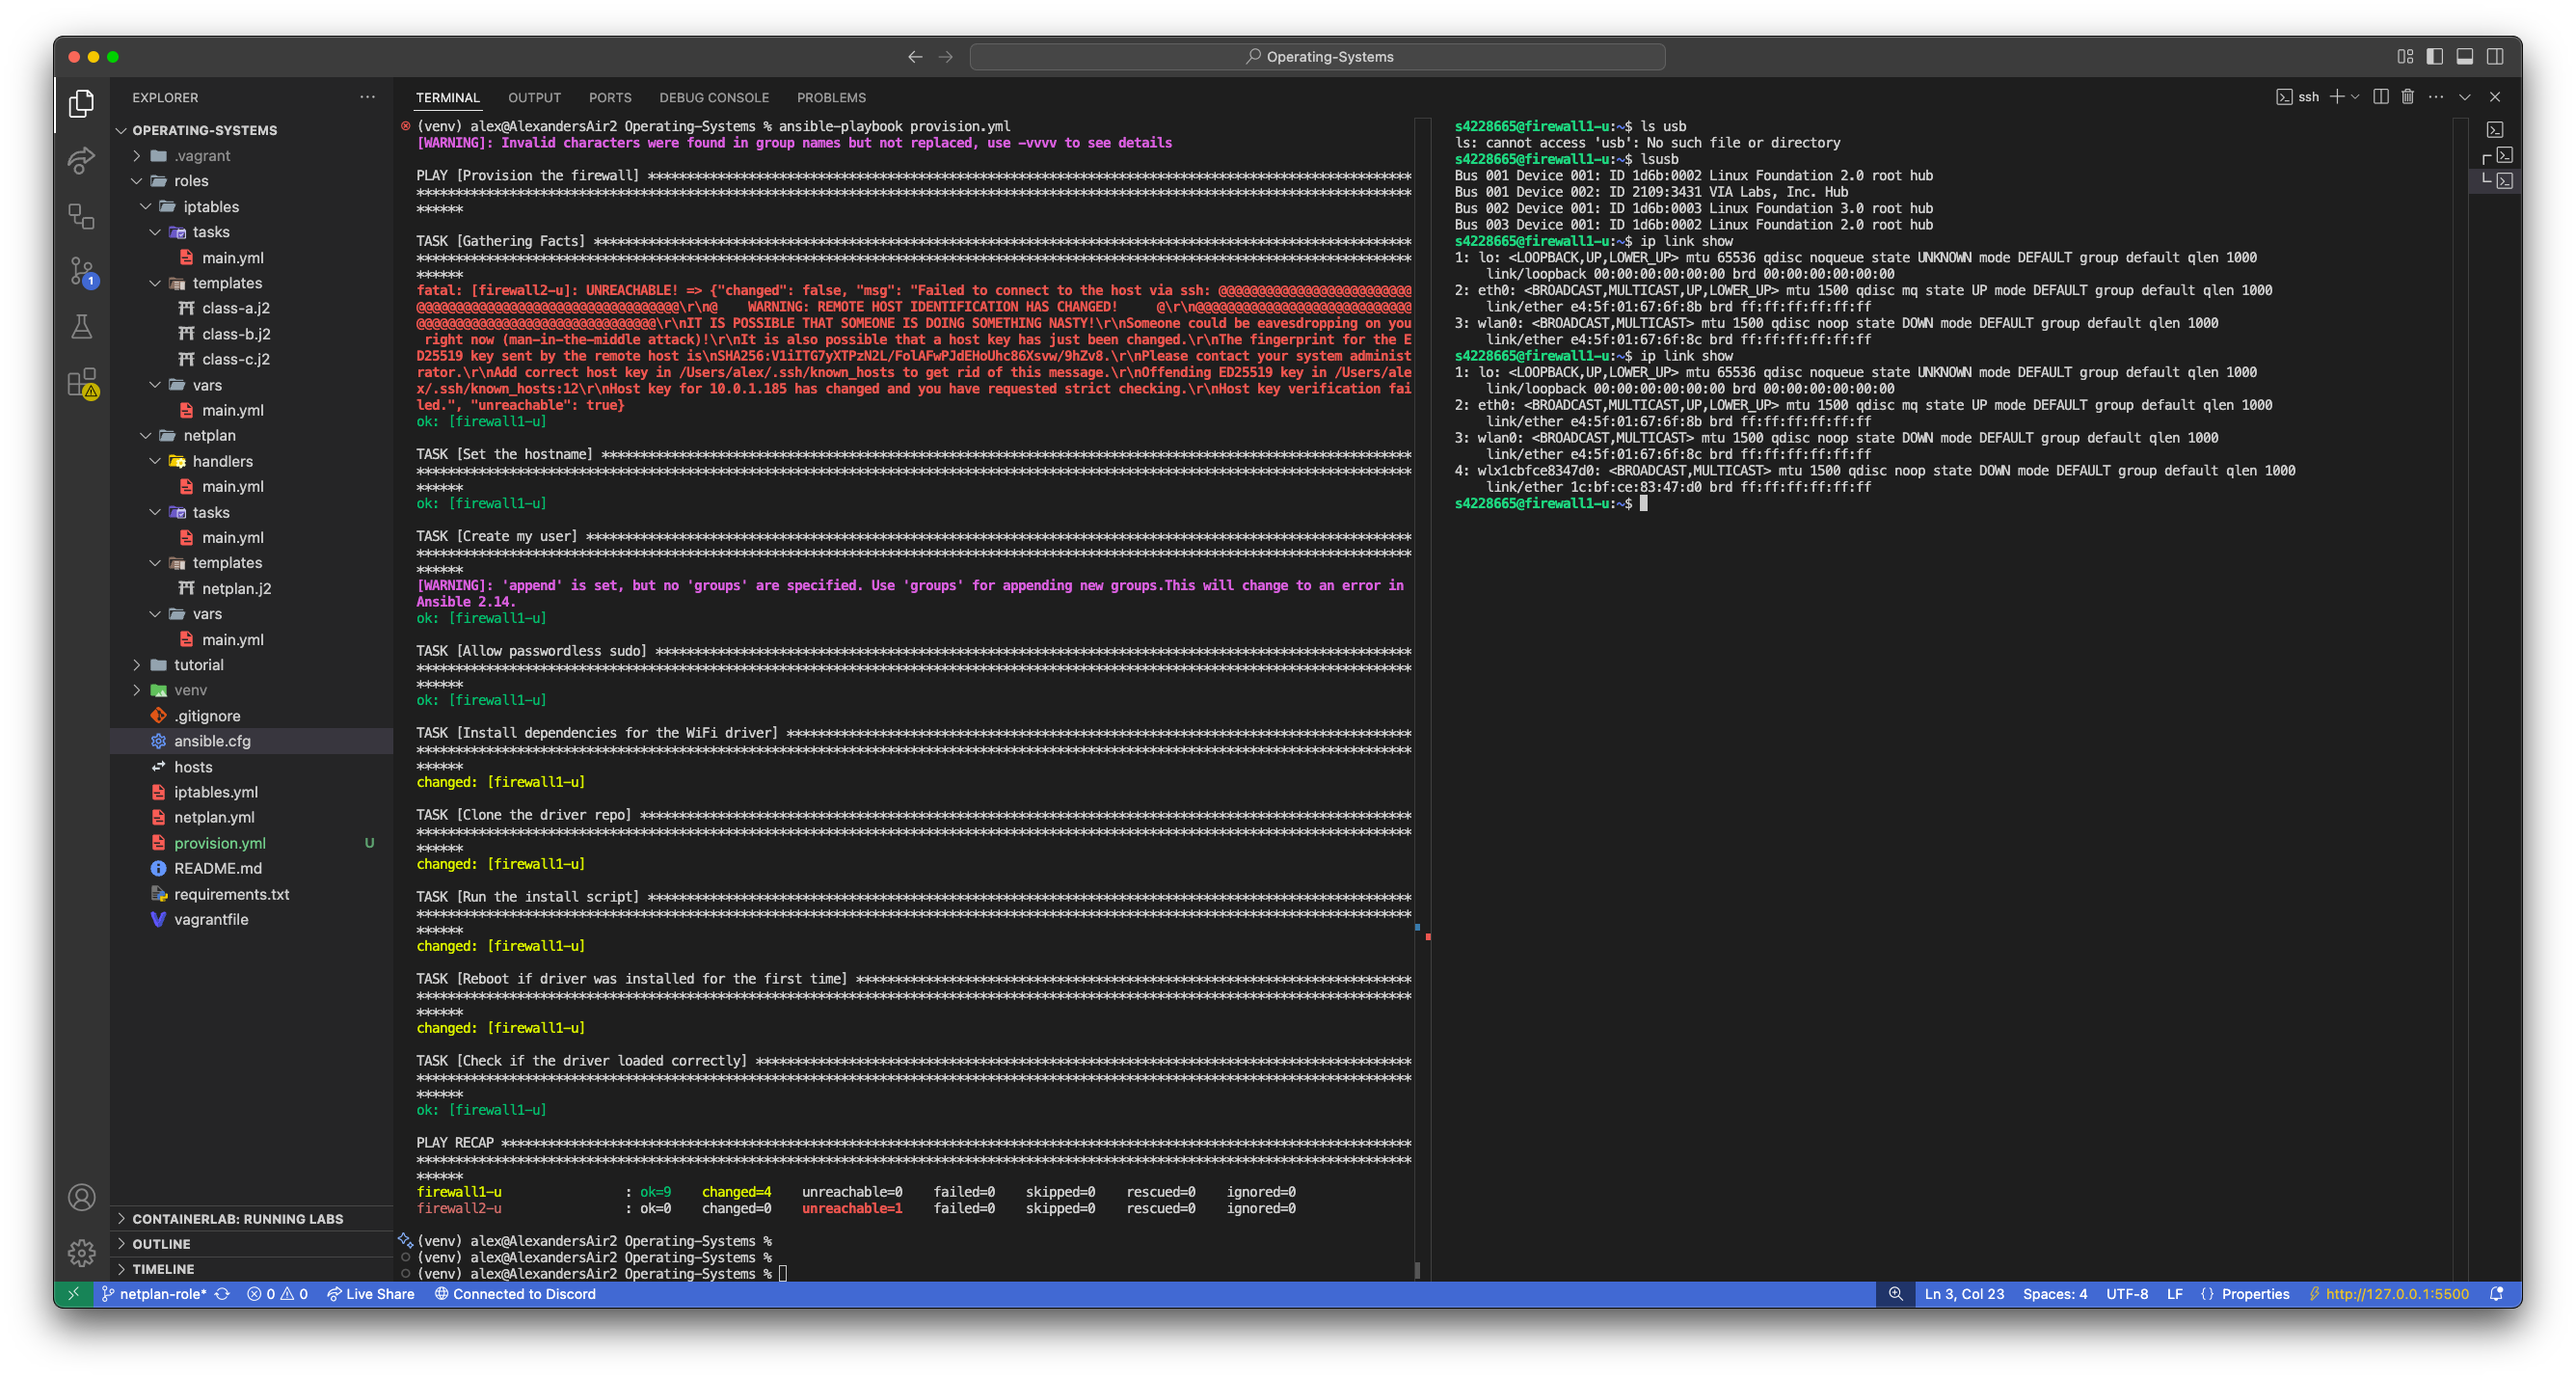
\includegraphics[width=\linewidth]{Screenshots/vscode-firewall-provision-validation.png}
    \caption{The output from bringing the provisioned VM with the driver up and it showing on the firewall}
    \label{vagrant:provision-firewall-nic}
\end{figure}

The output from \ref{vagrant:provision-vm-nic} shows the NIC is finally showing after unplugging and plugging the dongle back in after running the playbook. The interface came up as \verb|wlx1cbfce8347d0|. In adding to the playbook I had to go back and re-write it several times, namely because the driver interacts with the kernel so it needs to be compiled with Ubuntu's Dynamic Kernel Module Support (DKMS) package \parencite{Ubuntu2024DKMSDocumentation} so I needed to add the driver provided (by the VLE \parencite{Morrownr2024_8812au_Driver} but that didn't work). After installing it as intended nothing came up. 

I googled the output from \verb|lsusb| (figure \ref{fig:command-lsusb}) with drivers and the repo maintainer for both VLE suggested drivers as "Realtek c811 linux driver morrownr" and found a different (also unsupported) set of drivers \parencite{Morrownr2024_88x2bu_Driver} that worked.

\subsubsection{Multi-Interface Netplan Template}
\label{subsubsec:netplan-template}

The netplan configuration template (Figure \ref{code:ansible-netplan-template}) defines all three network interfaces with static IP addressing, DNS configuration, and routing rules.

\begin{figure}[H]
    \centering
    \begin{minted}{YAML}
    Nah, I'd win
    \end{minted}
    \caption{The jinja2 template used for configuring the interfaces}
    \label{code:ansible-netplan-template}
\end{figure}

In testing this on the VM firewall (with variables from figure \ref{fig:netplan-vars} and deploying in figure \ref{vagrant:netplan-deploy}), I noticed this won't work as well as the real firewall as the hardware setup isn't the same. While having a virtual machine (an easily destructible testing environment) is good for validating config changes, there are limitations.

\begin{figure}[H]
    \centering
    \begin{minted}{YAML}
    Nah, I'd win
    \end{minted}
    \caption{The Jinja2 template used for configuring the interfaces}
    \label{code:ansible-netplan-vars}
\end{figure}

\begin{figure}[H]
    \centering
    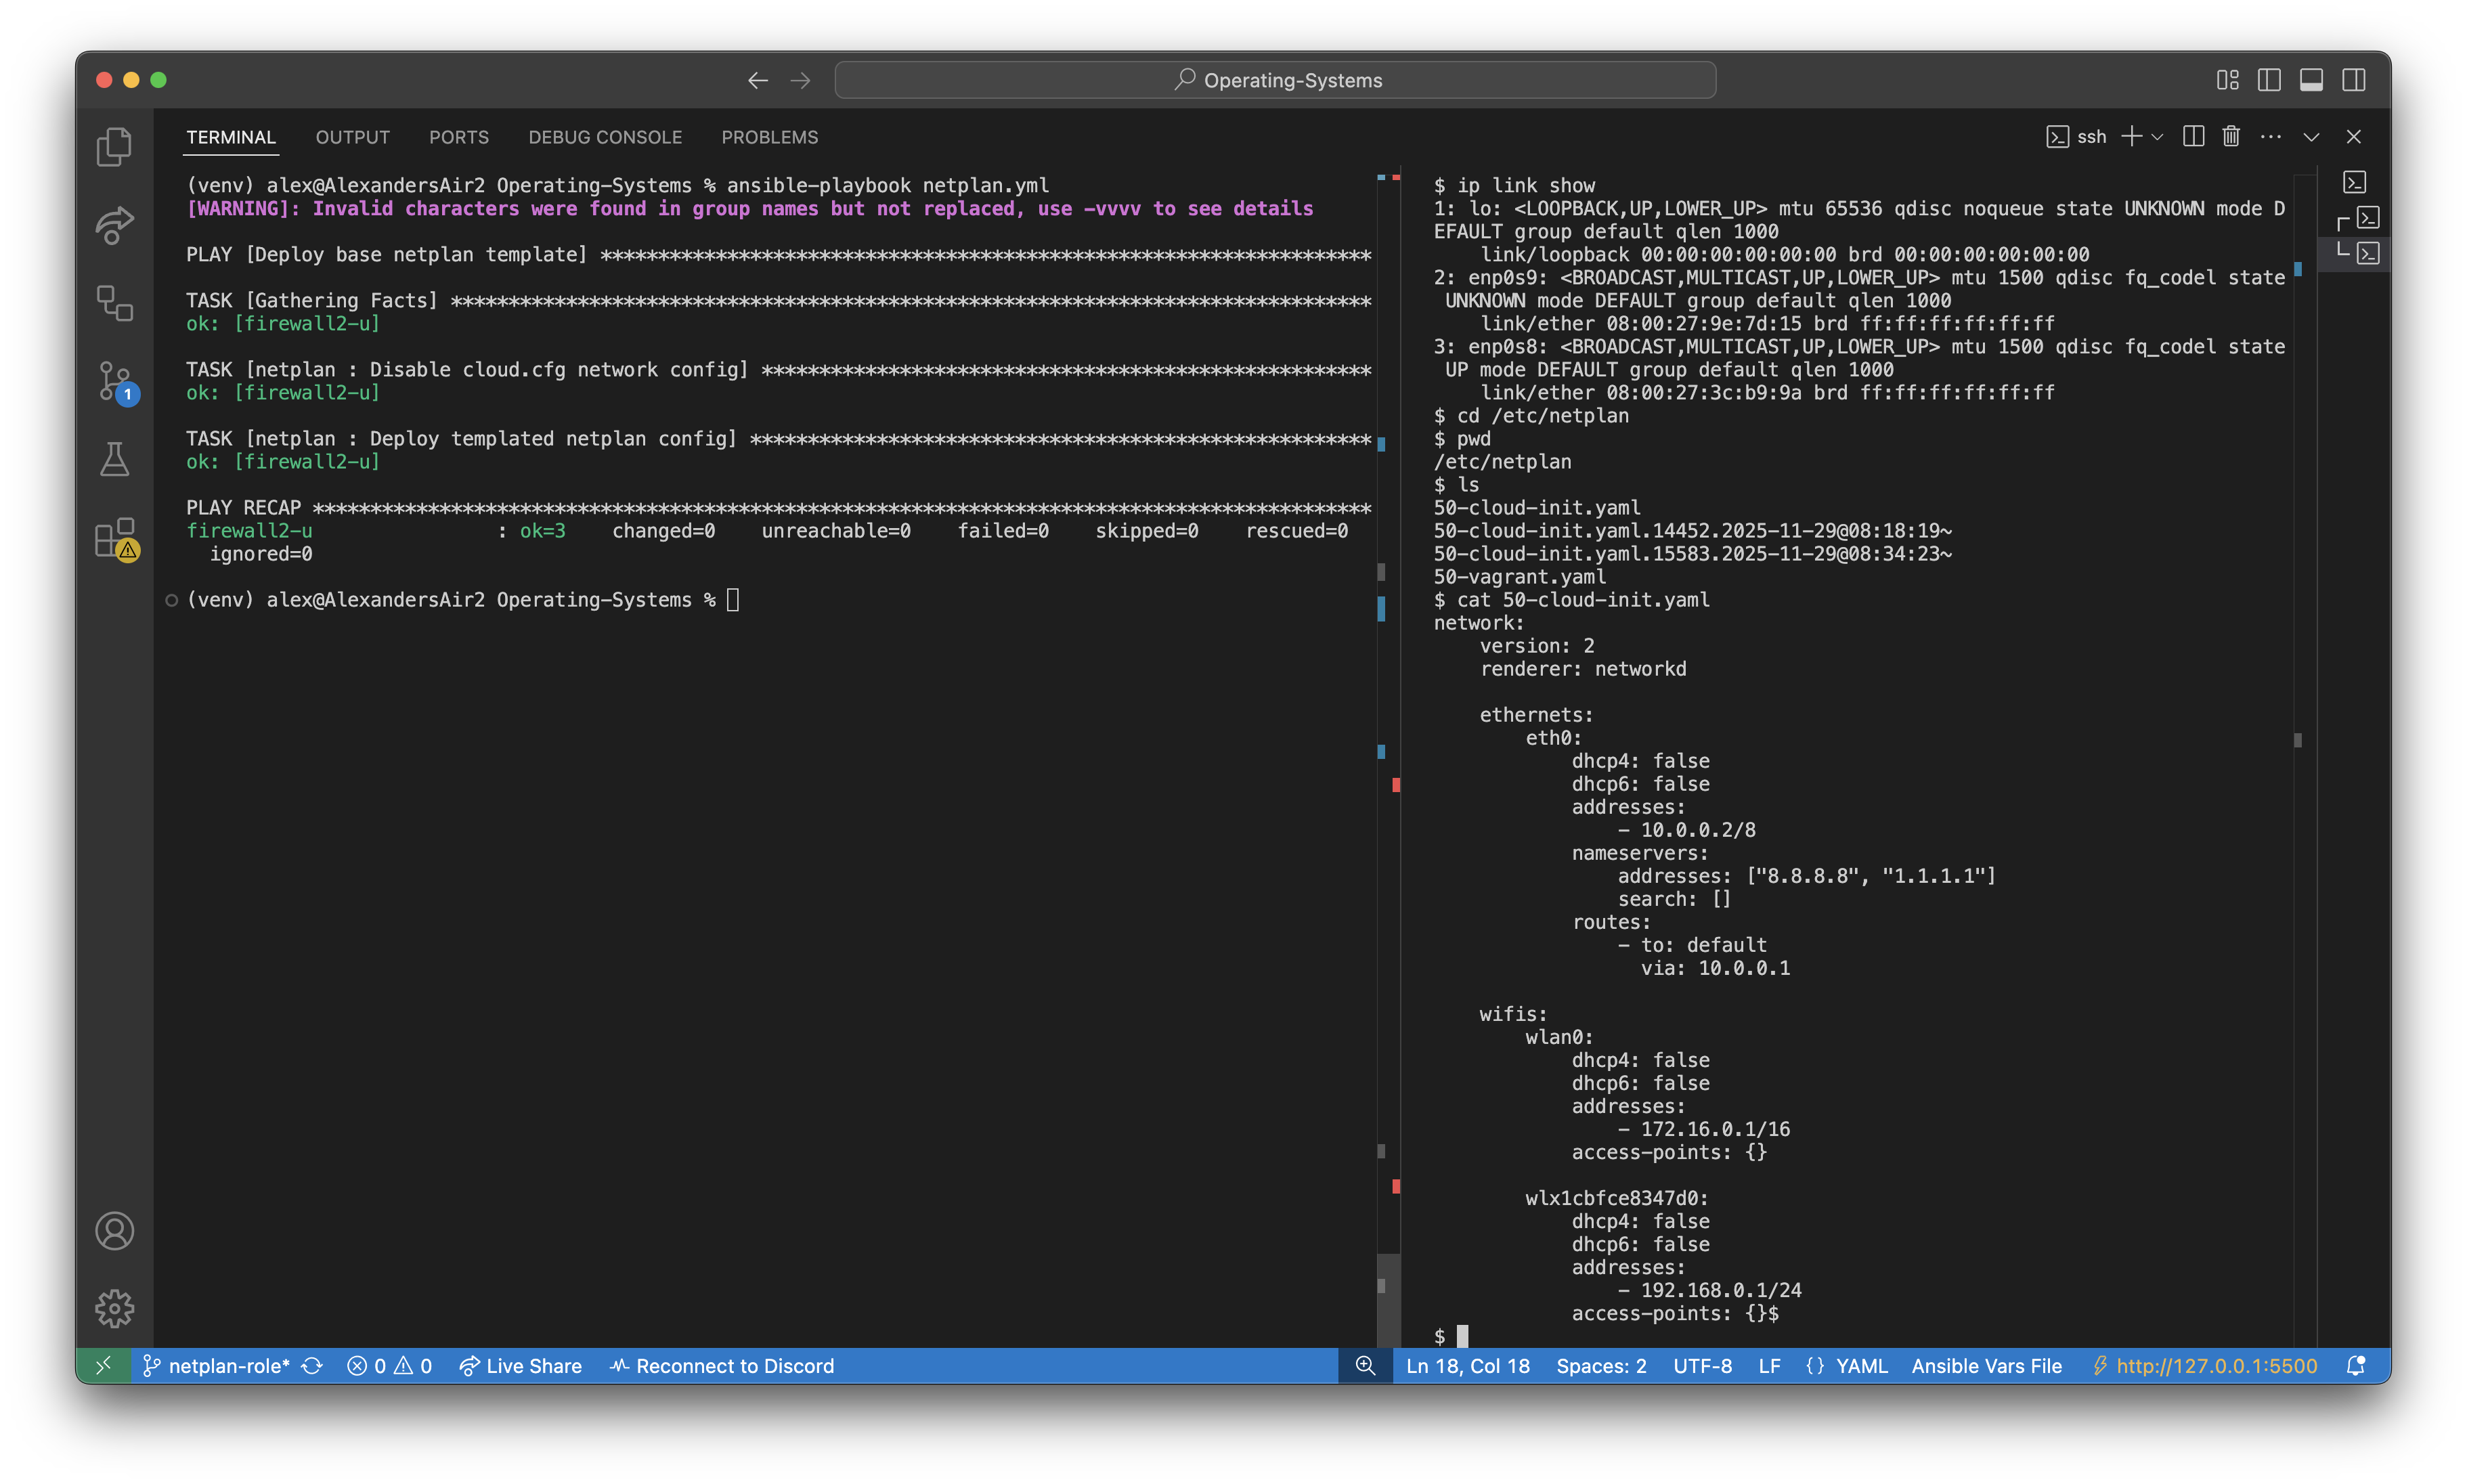
\includegraphics[width=1\linewidth]{Screenshots/vscode-vagrant-netplan-deploy.png}
    \caption{Side by side viewing of the successful netplan deploy (left) and the applied netplan config (right)}
    \label{vagrant:netplan-deploy}
\end{figure}

As the deploy was validated on the VM, the config can be deployed to the firewall.

\begin{figure}[H]
    \centering
    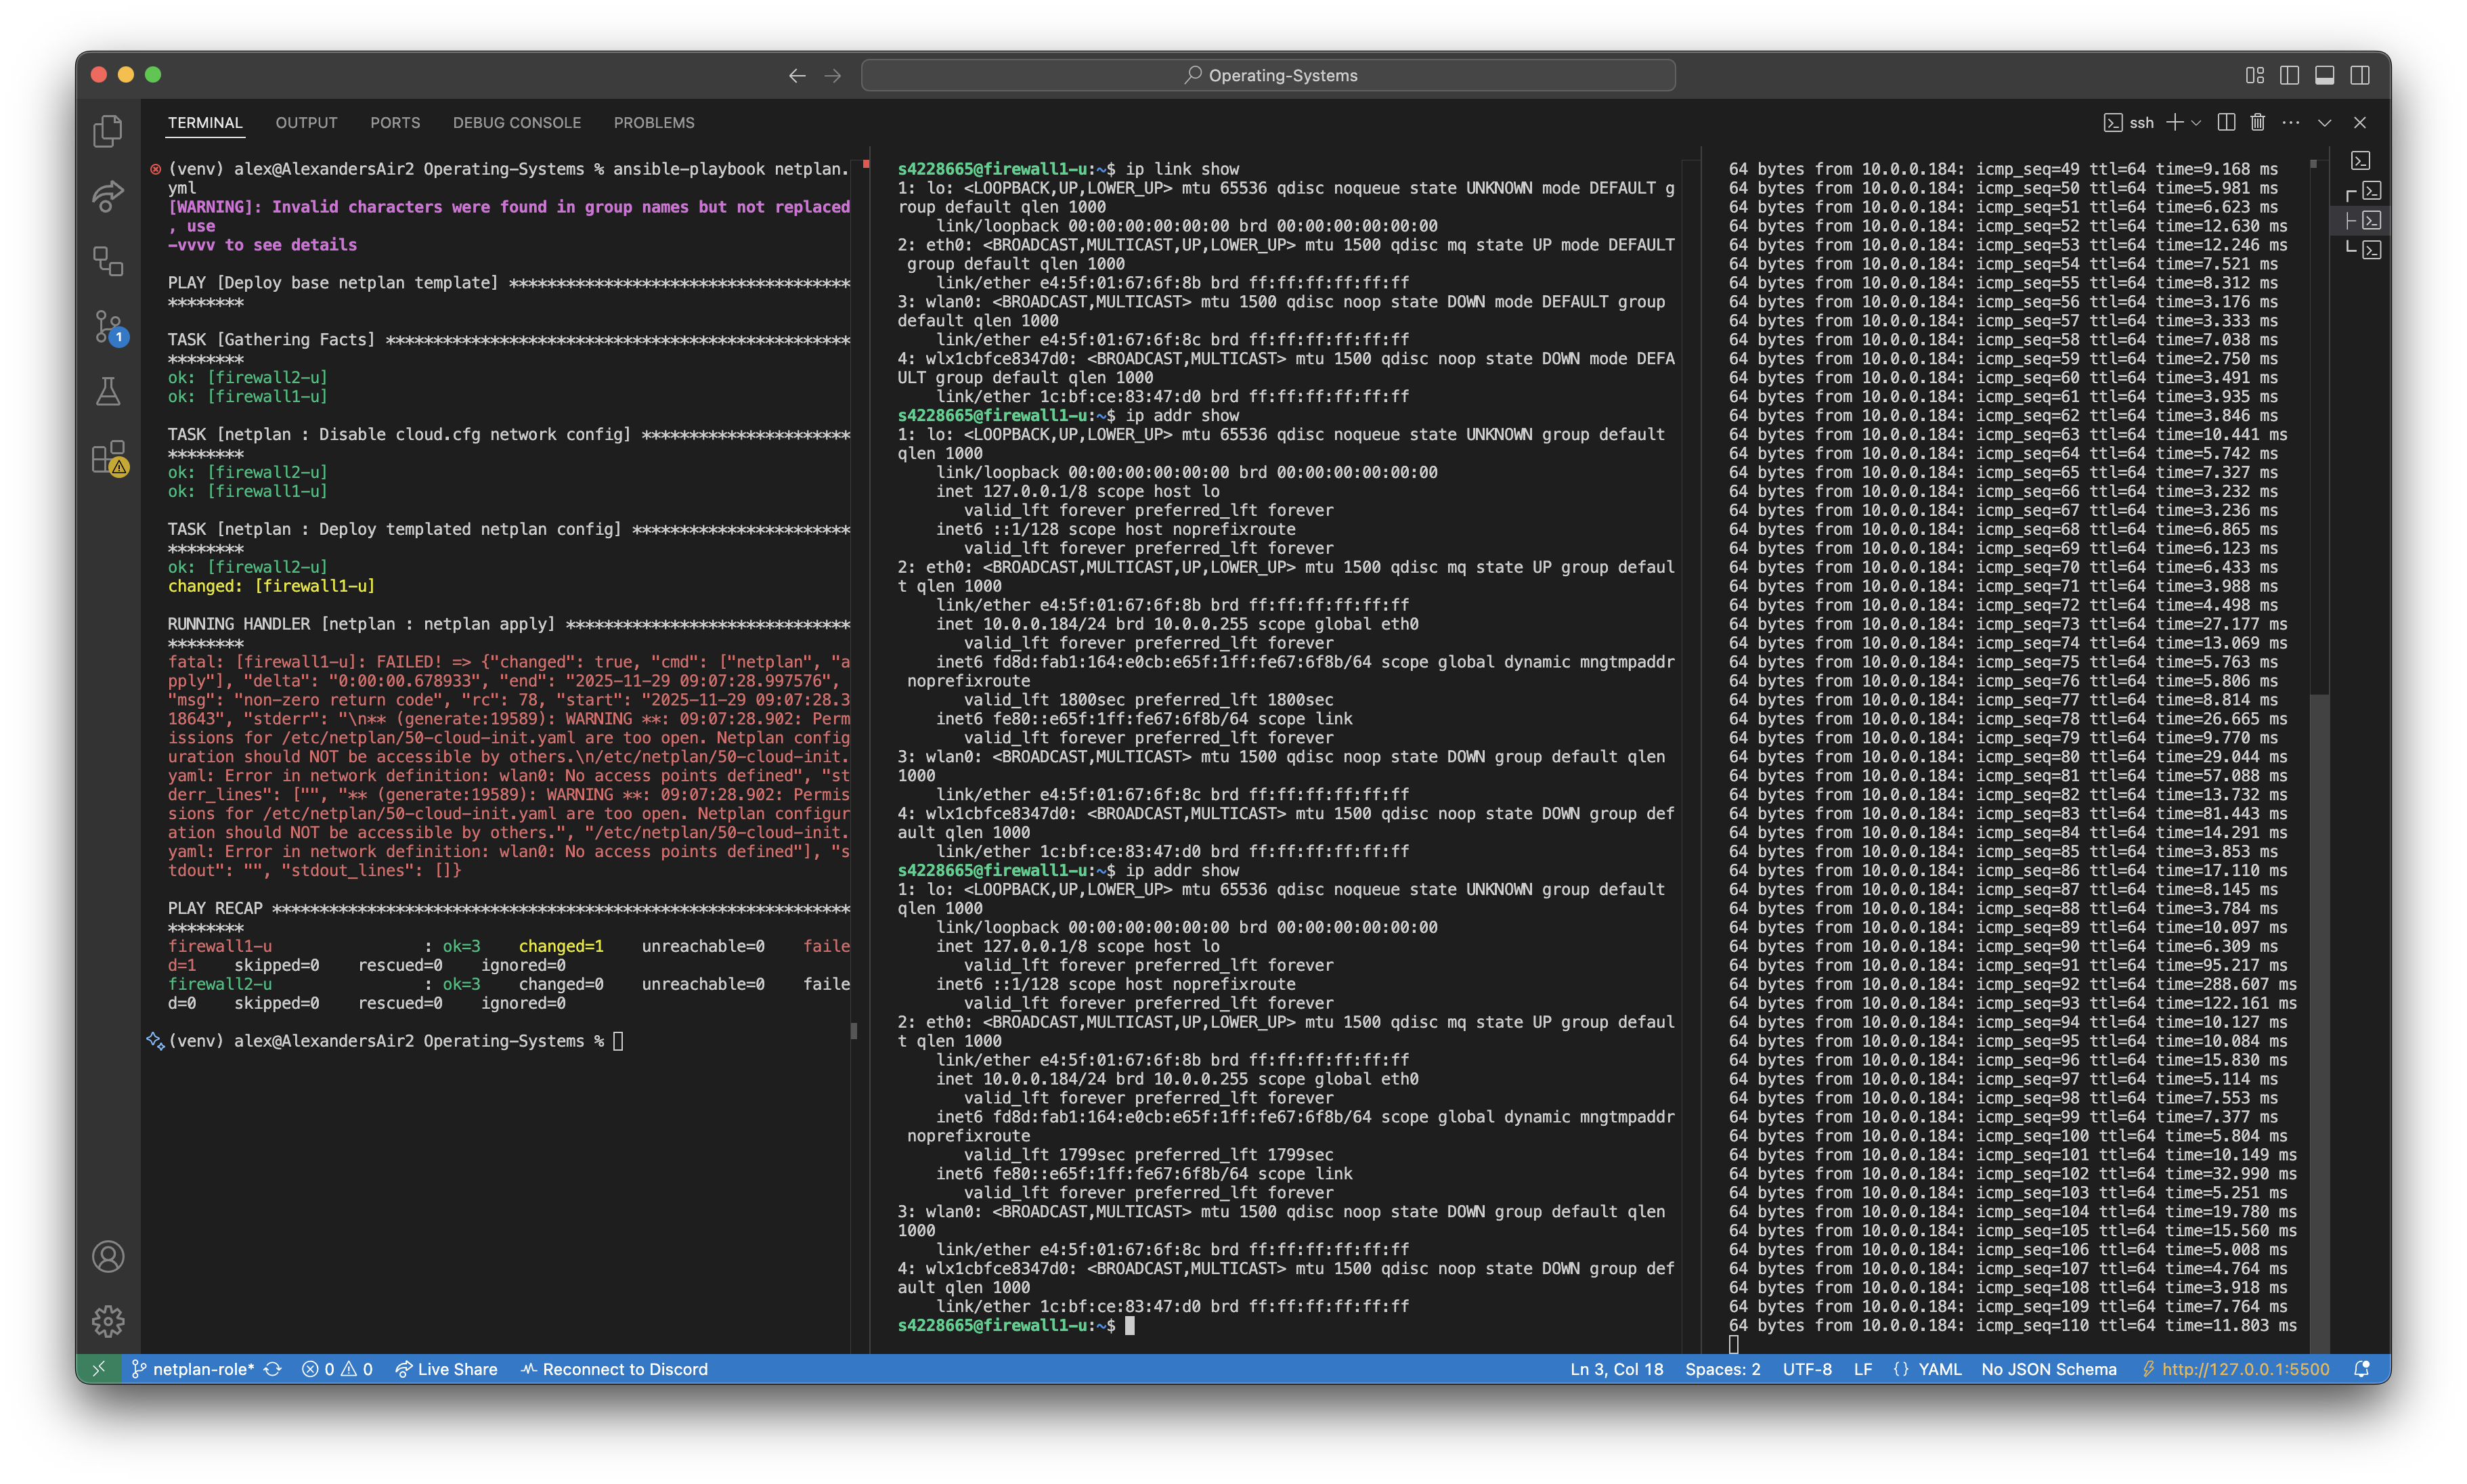
\includegraphics[width=1\linewidth]{Screenshots/vscode-both-neplan-deploy.png}
    \caption{View of the deploy to both firewalls (left), a SSH session to the firewall showing the before and after states of the netplan deploy (centre) and a running ping to confirm if something went wrong while deploying the config (right)}
    \label{fig:combined-netplan-deploy}
\end{figure}

The centre part of figure \ref{fig:combined-netplan-deploy} shows the two NICs as down, after trying to bring them up manually I realised they need to be configured as access-points, not as WiFi clients. Netplan doesn't support this but hostapd \parencite{LinuxKernel2024HostapdDocumentation} \parencite{Hostapd2024Documentation} does.

On Linux operating systems, WiFi interfaces being used as access points (APs) need the hostapd daemon to manage client authentication, and beacon broadcasting \parencite{Hostapd2024Documentation}. Netplan configures IP addressing and routing at the network layer (Layer 3), but hostapd operates at the data link and physical layers (Layers 1 and 2) to establish the wireless medium.

To use hostapd (with logging), you need to use systemd services \parencite{Freedesktop2024Systemd} to give a level of persistence via \texttt{WantedBy=multi-user.target}. A systemd service will enable the hostapd daemons to start after network initialisation (\texttt{After=network.target}) and automatically restart on failure (\texttt{Restart=on-failure}). This isn't needed for netplan or iptables as netplan is persistant and iptables uses an additional module (REFERNECE TO IPTABLESROLE PERSISTANCE) to keep the config active.

As hostapd can be defined as systemd services, it fits nicely into the Ansible IaC approach, as this can be sorted into a new role defined as figure \ref{fig:ansible-hostapd-role}.

\begin{figure}[H]
    \centering
    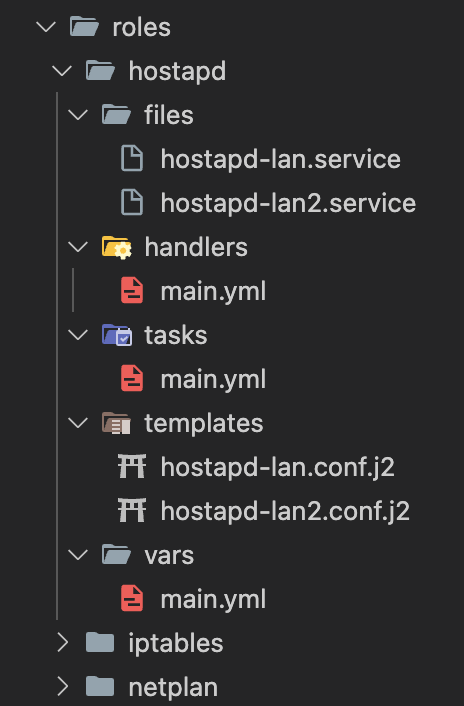
\includegraphics[width=0.5\linewidth]{Screenshots/vscode-hostapd-role.png}
    \caption{The new role structure for hostapd}
    \label{fig:ansible-hostapd-role}
\end{figure}

. This architecture follows established patterns for Raspberry Pi wireless access point deployment \parencite{RaspberryPi2024Documentation}, separating Layer 2 wireless management (hostapd) from Layer 3 network configuration (netplan) for modular, maintainable infrastructure automation.

\begin{figure}[H]
    \centering
    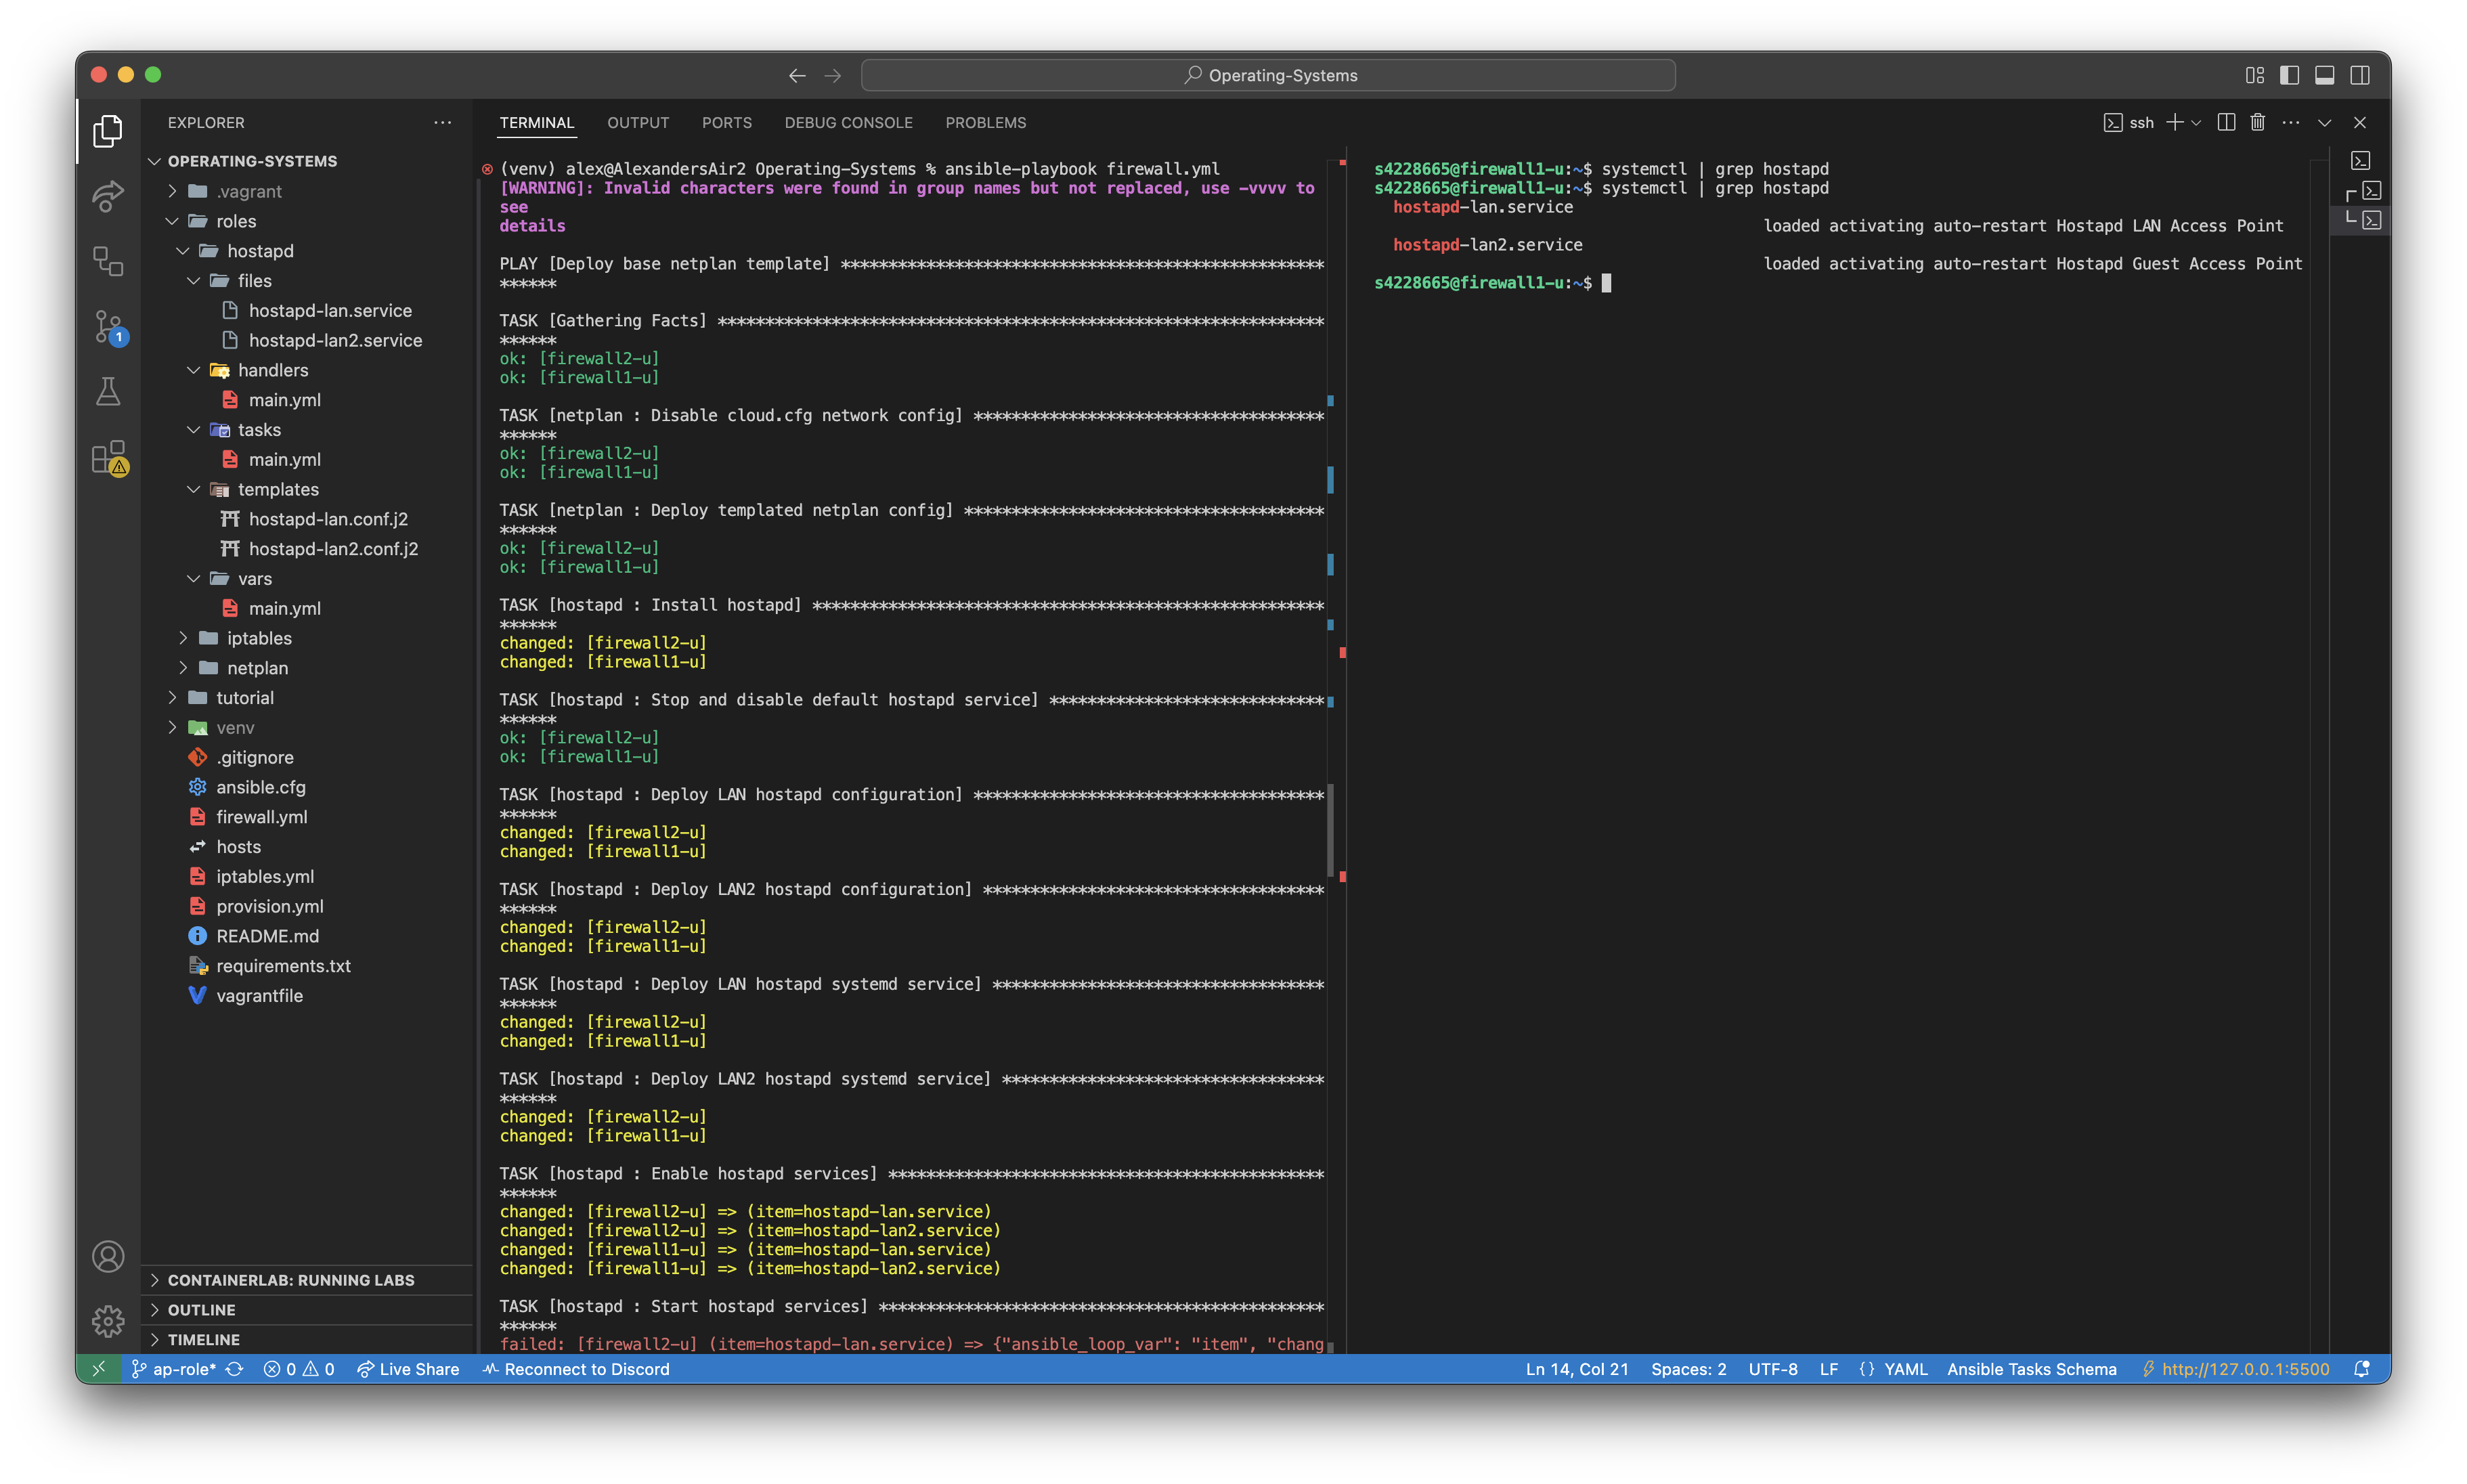
\includegraphics[width=1\linewidth]{Screenshots/vscode-both-hostapd-deploy.png}
    \caption{First deploy of the hostapd role (left) and the services running on the firewall (right)}
    \label{fig:ansible-hostapd-deploy}
\end{figure}


\begin{figure}[H]
    \centering
    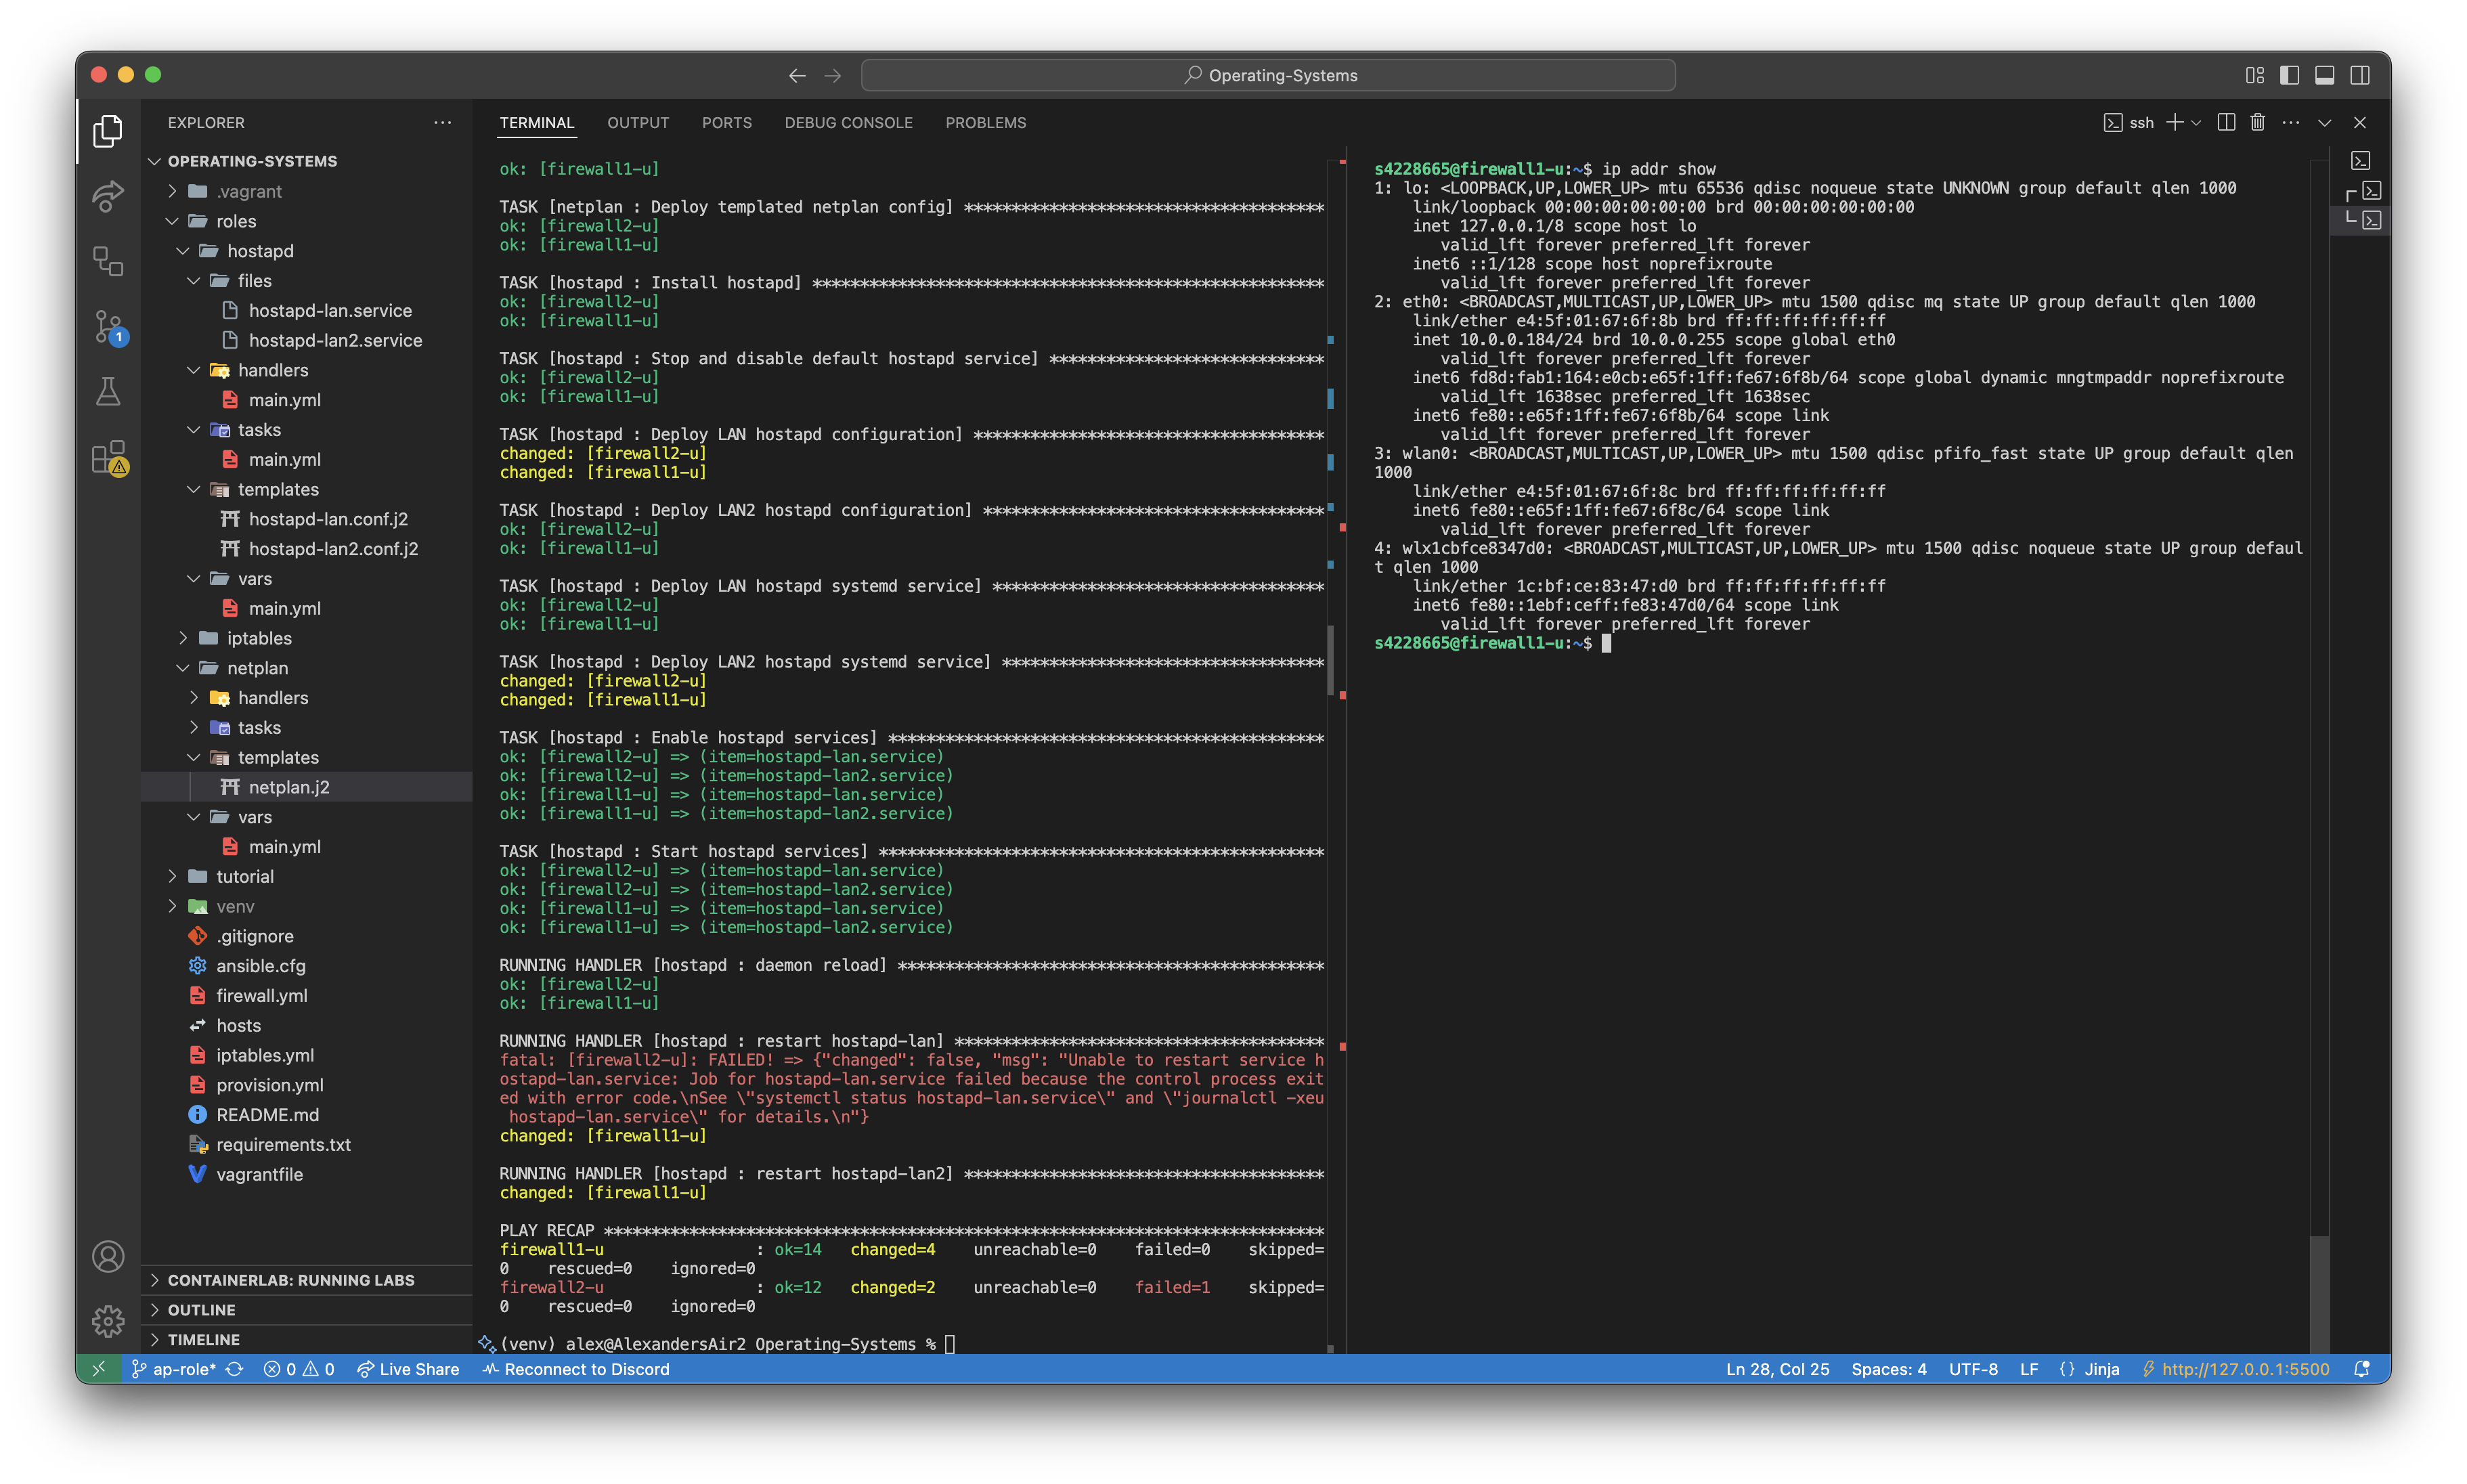
\includegraphics[width=1\linewidth]{Screenshots/vscode-both-hostapd-deploy2.png}
    \caption{Enter Caption}
    \label{fig:placeholder}
\end{figure}

Something something the 5G SSID was showing up but not the 2.4G one, and it could be related to one of the handlers failing on the main firewall - this is expected on the VM as it's not running on the hardware, at this point I decided to start changing the netplan + hostapd config, the extent of which can be seen in this pull request (REFERNECE PULL REQUEST WITH CHANGES). To validate the changes, I worked from my laptop and the VM firewall (figure \ref{fig:ansible-hostapd+netplan-deploy-test}).

\begin{figure}[H]
    \centering
    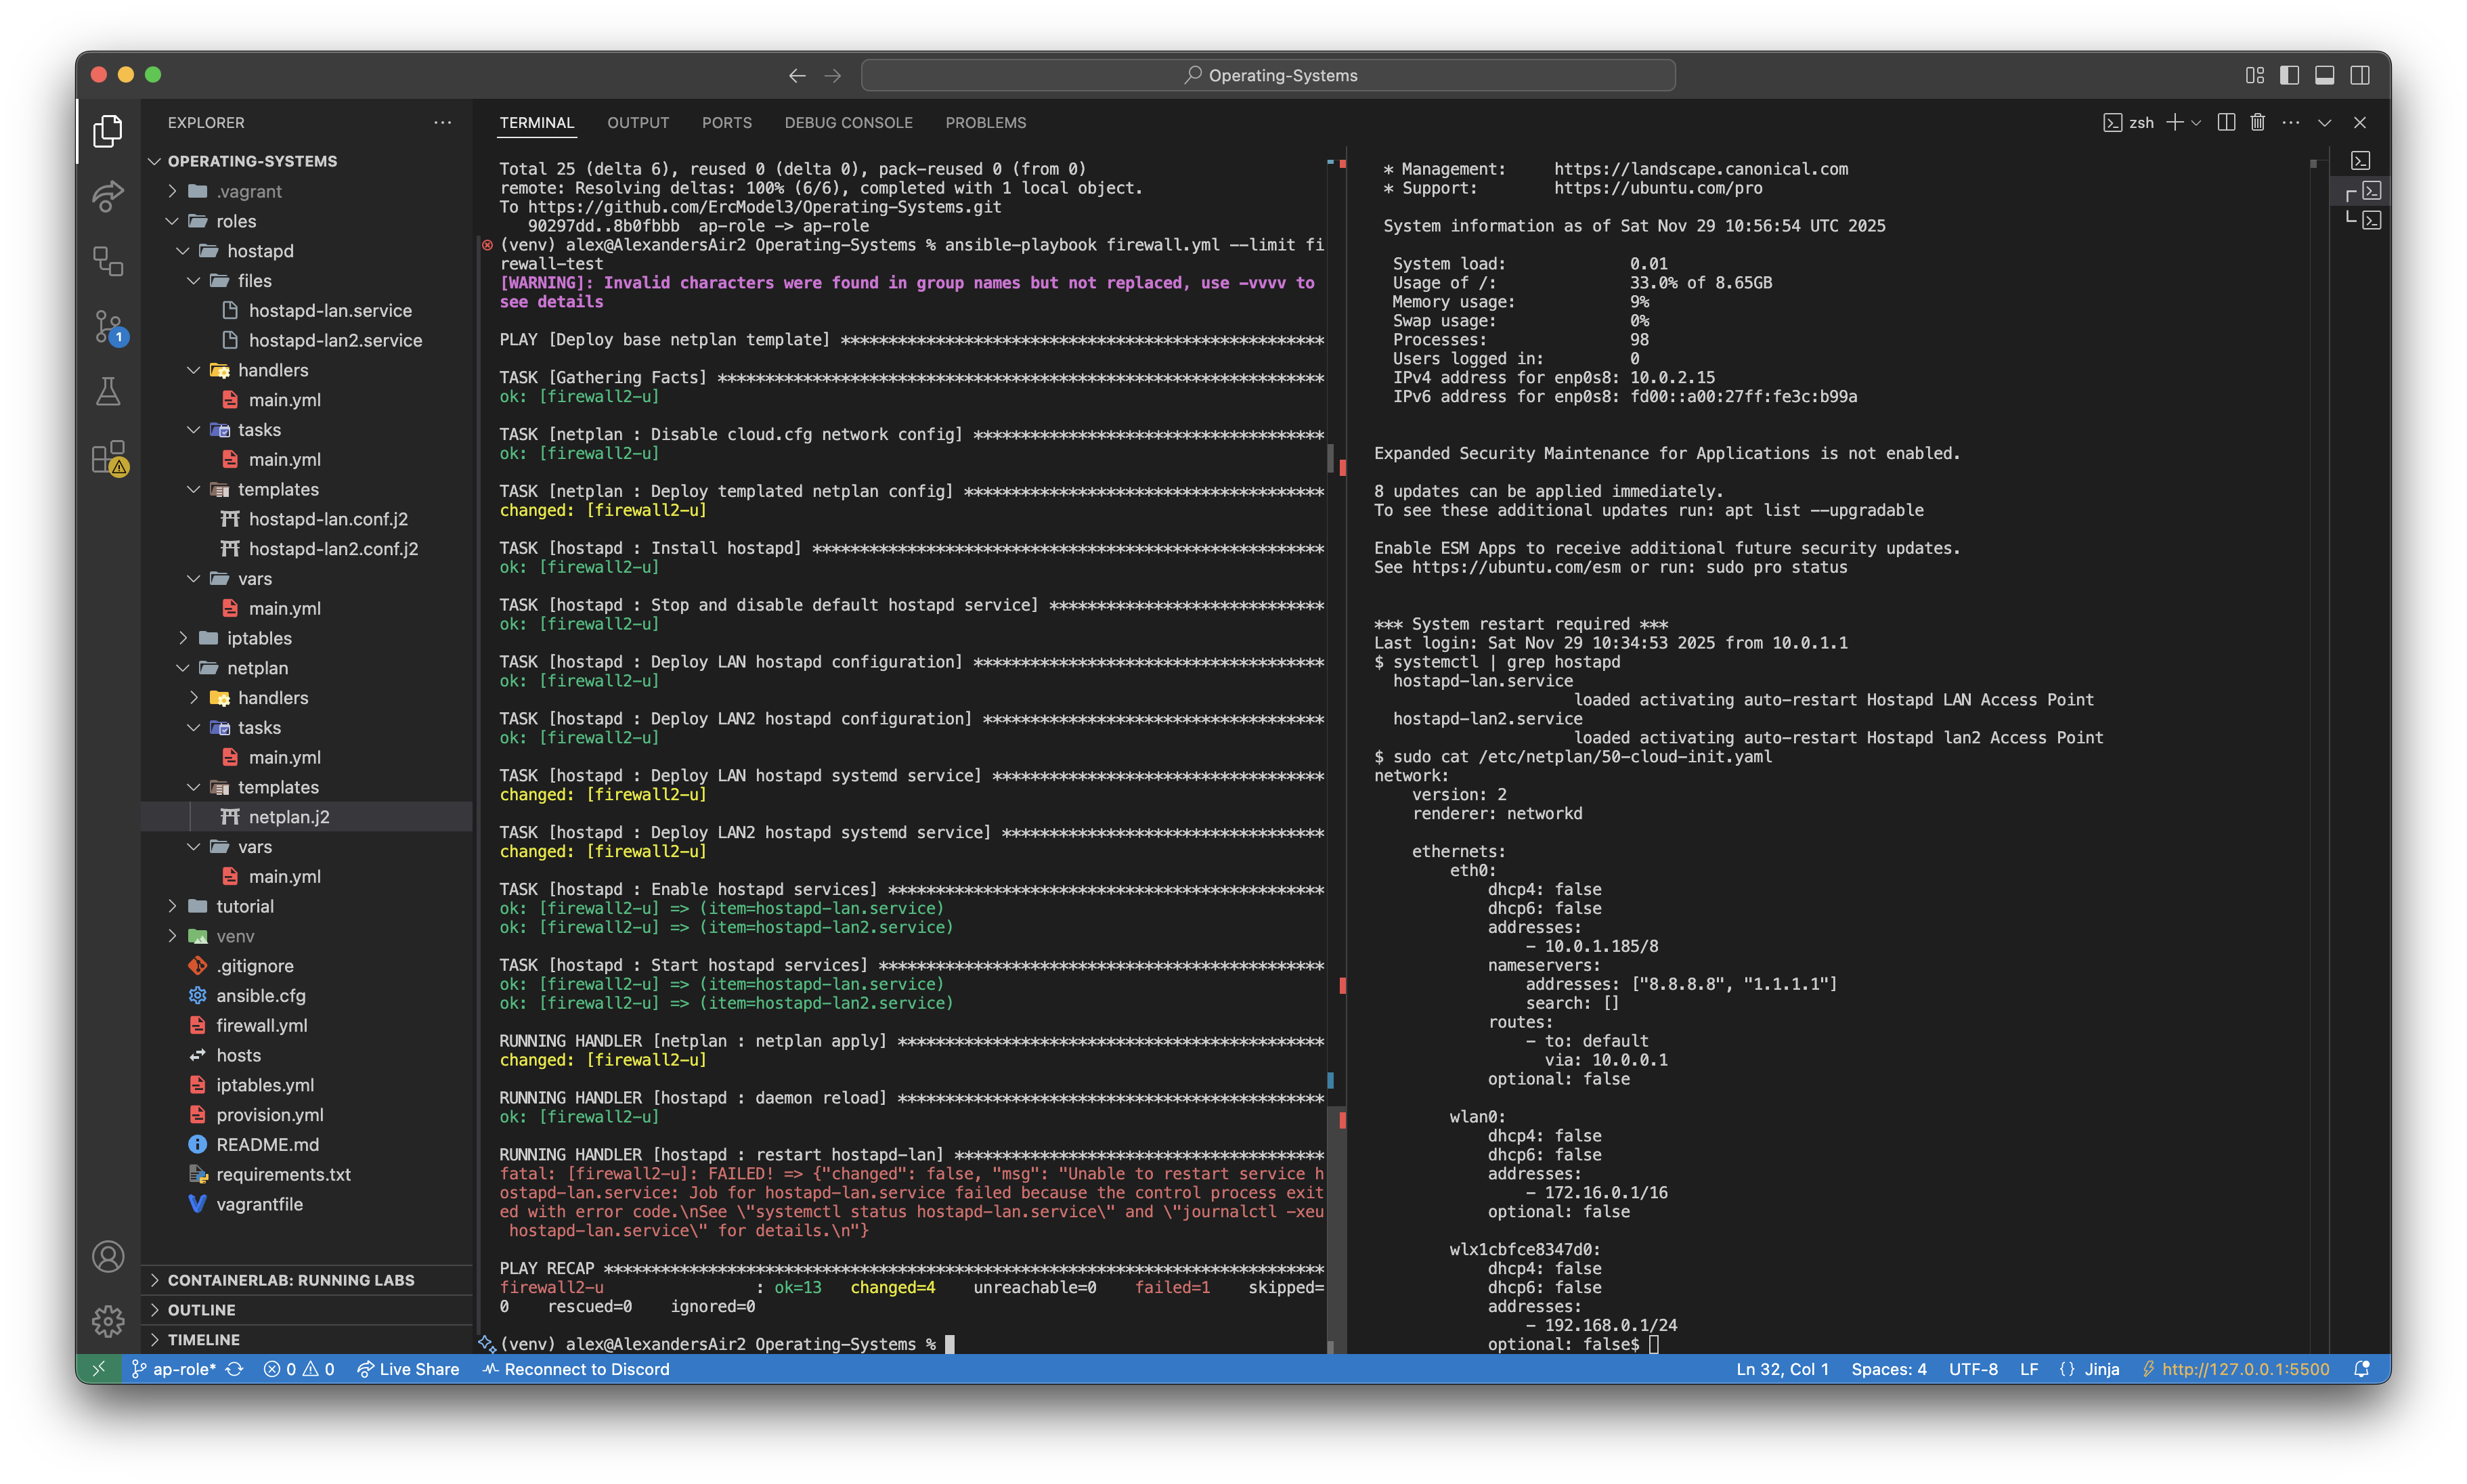
\includegraphics[width=1\linewidth]{Screenshots/image.png}
    \caption{Enter Caption}
    \label{fig:ansible-hostapd+netplan-deploy-test}
\end{figure}

And after a successful deploy, it was time to push it to the firewall (figure \ref{fig:ansible-hostapd+netplan-deploy-prod}).

\begin{figure}[H]
    \centering
    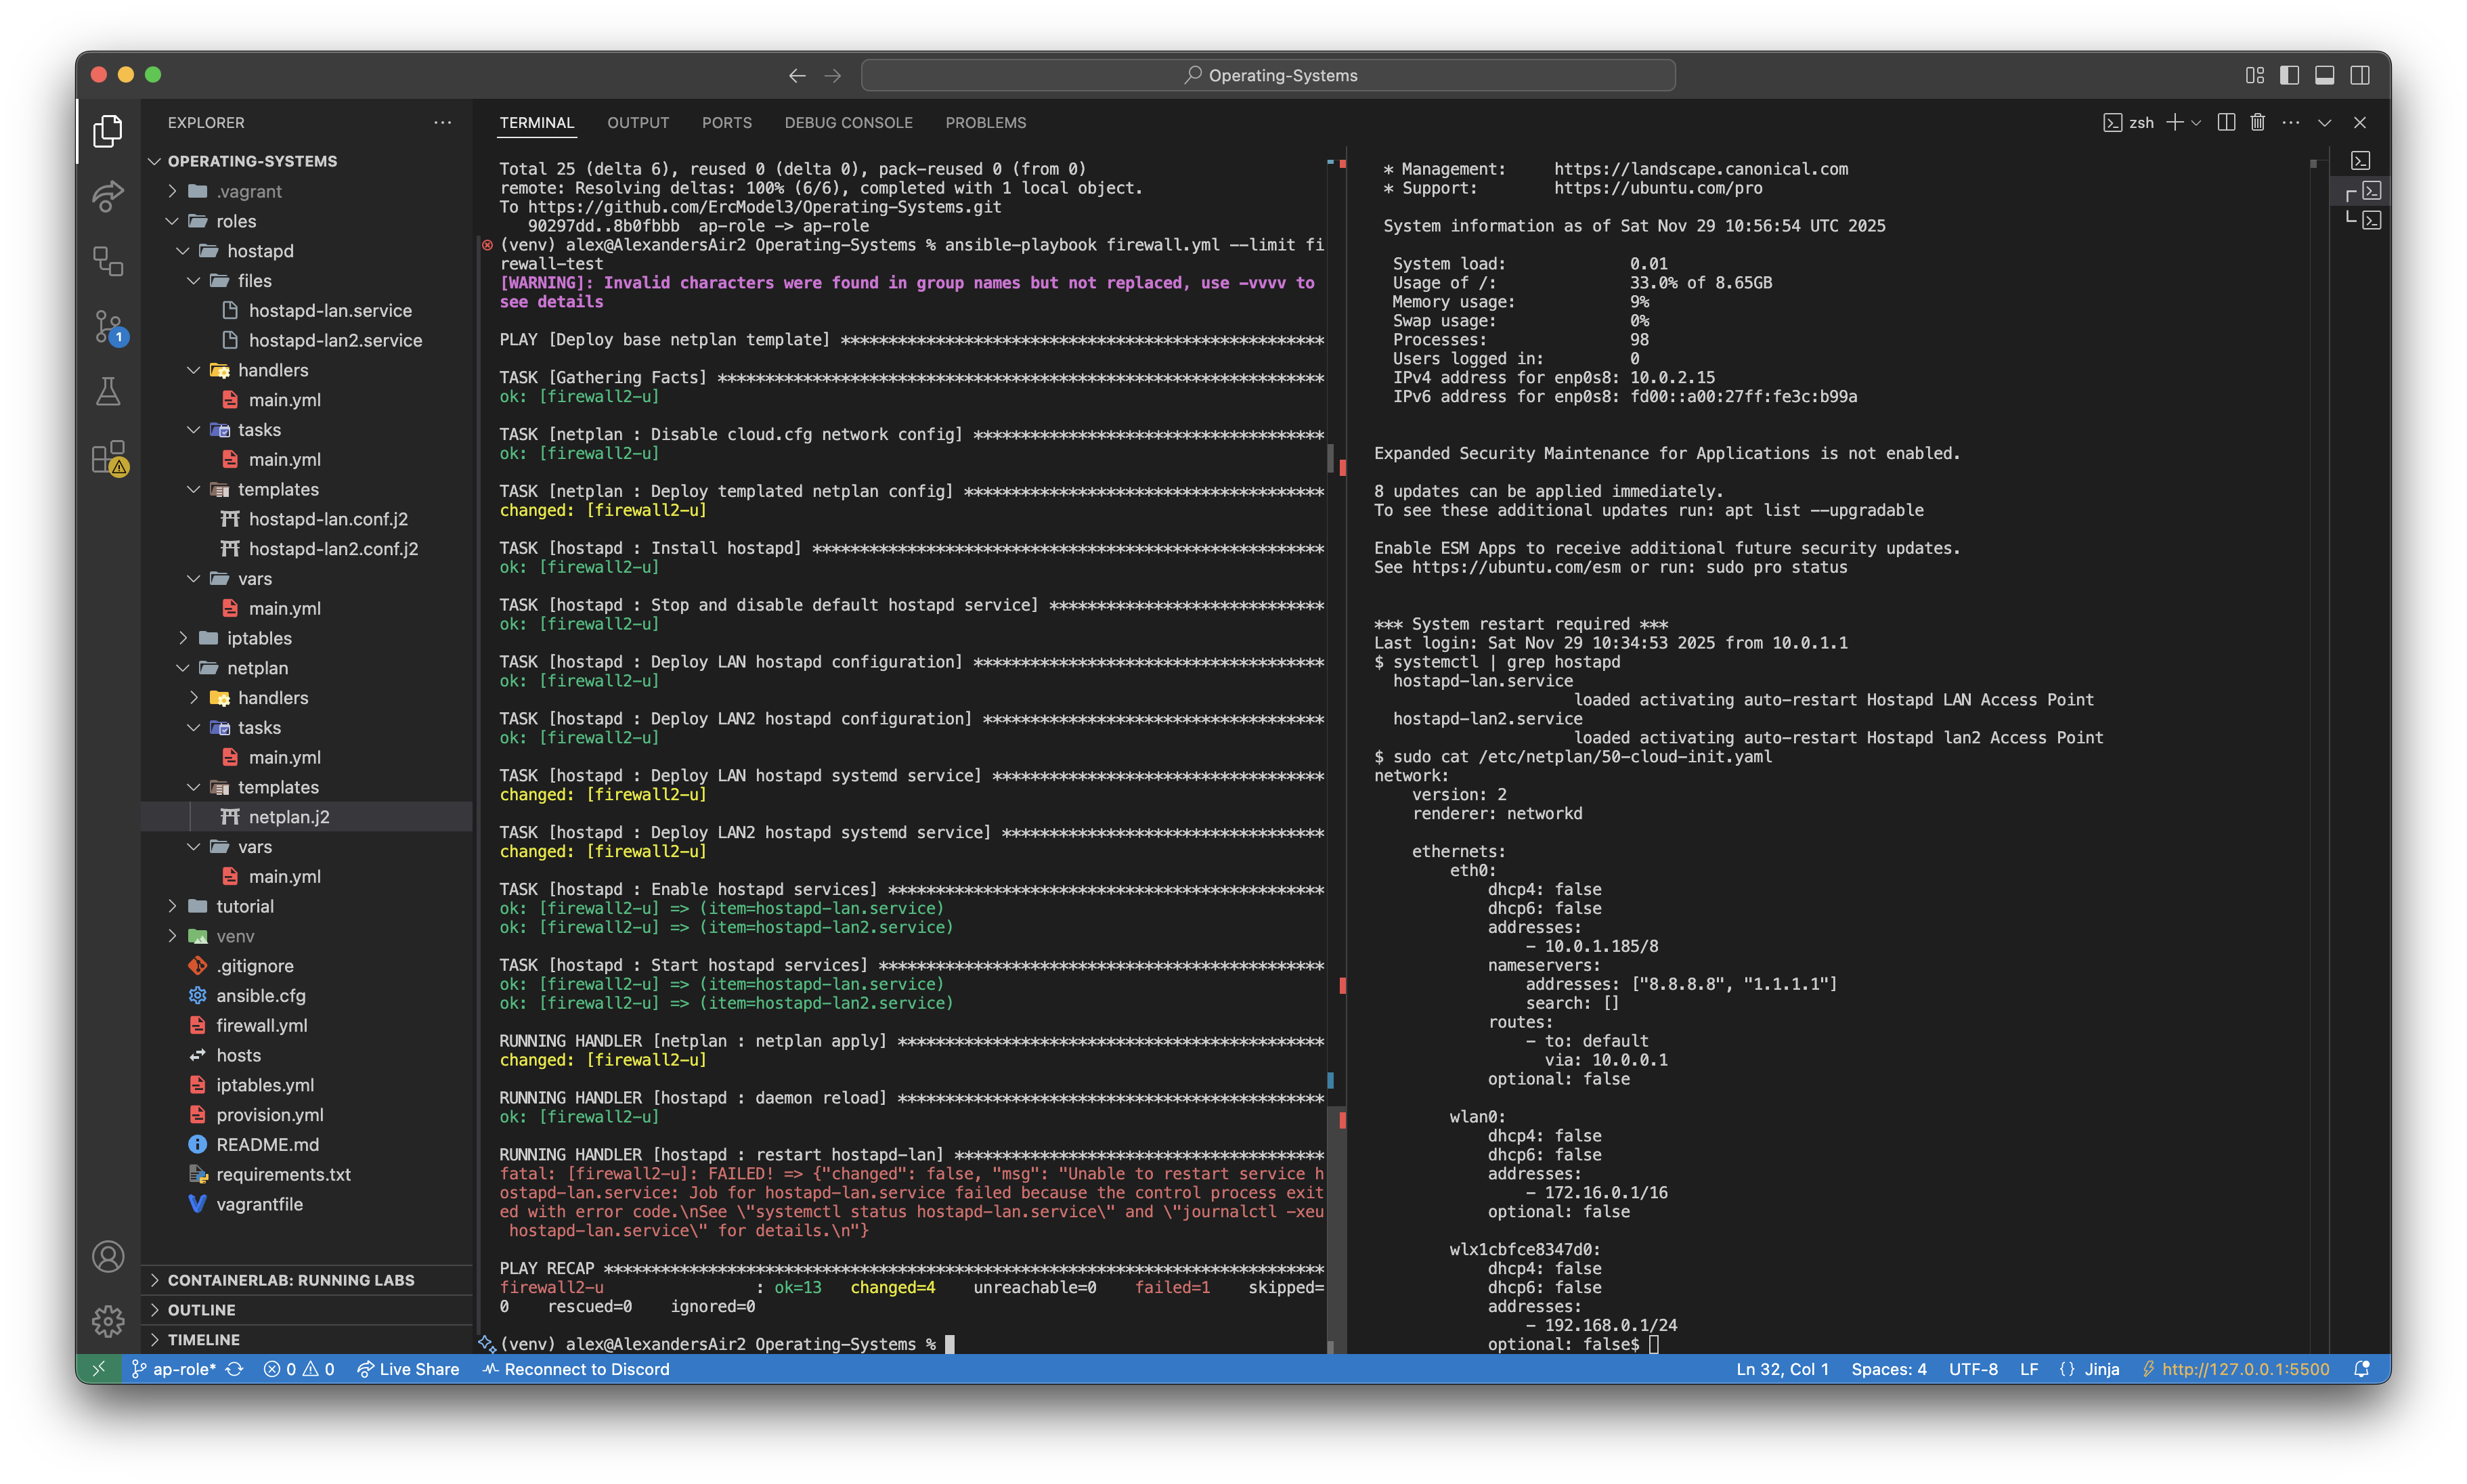
\includegraphics[width=1\linewidth]{Screenshots/image.png}
    \caption{Enter Caption}
    \label{fig:ansible-hostapd+netplan-deploy-prod}
\end{figure}

\begin{figure}[H]
    \centering
    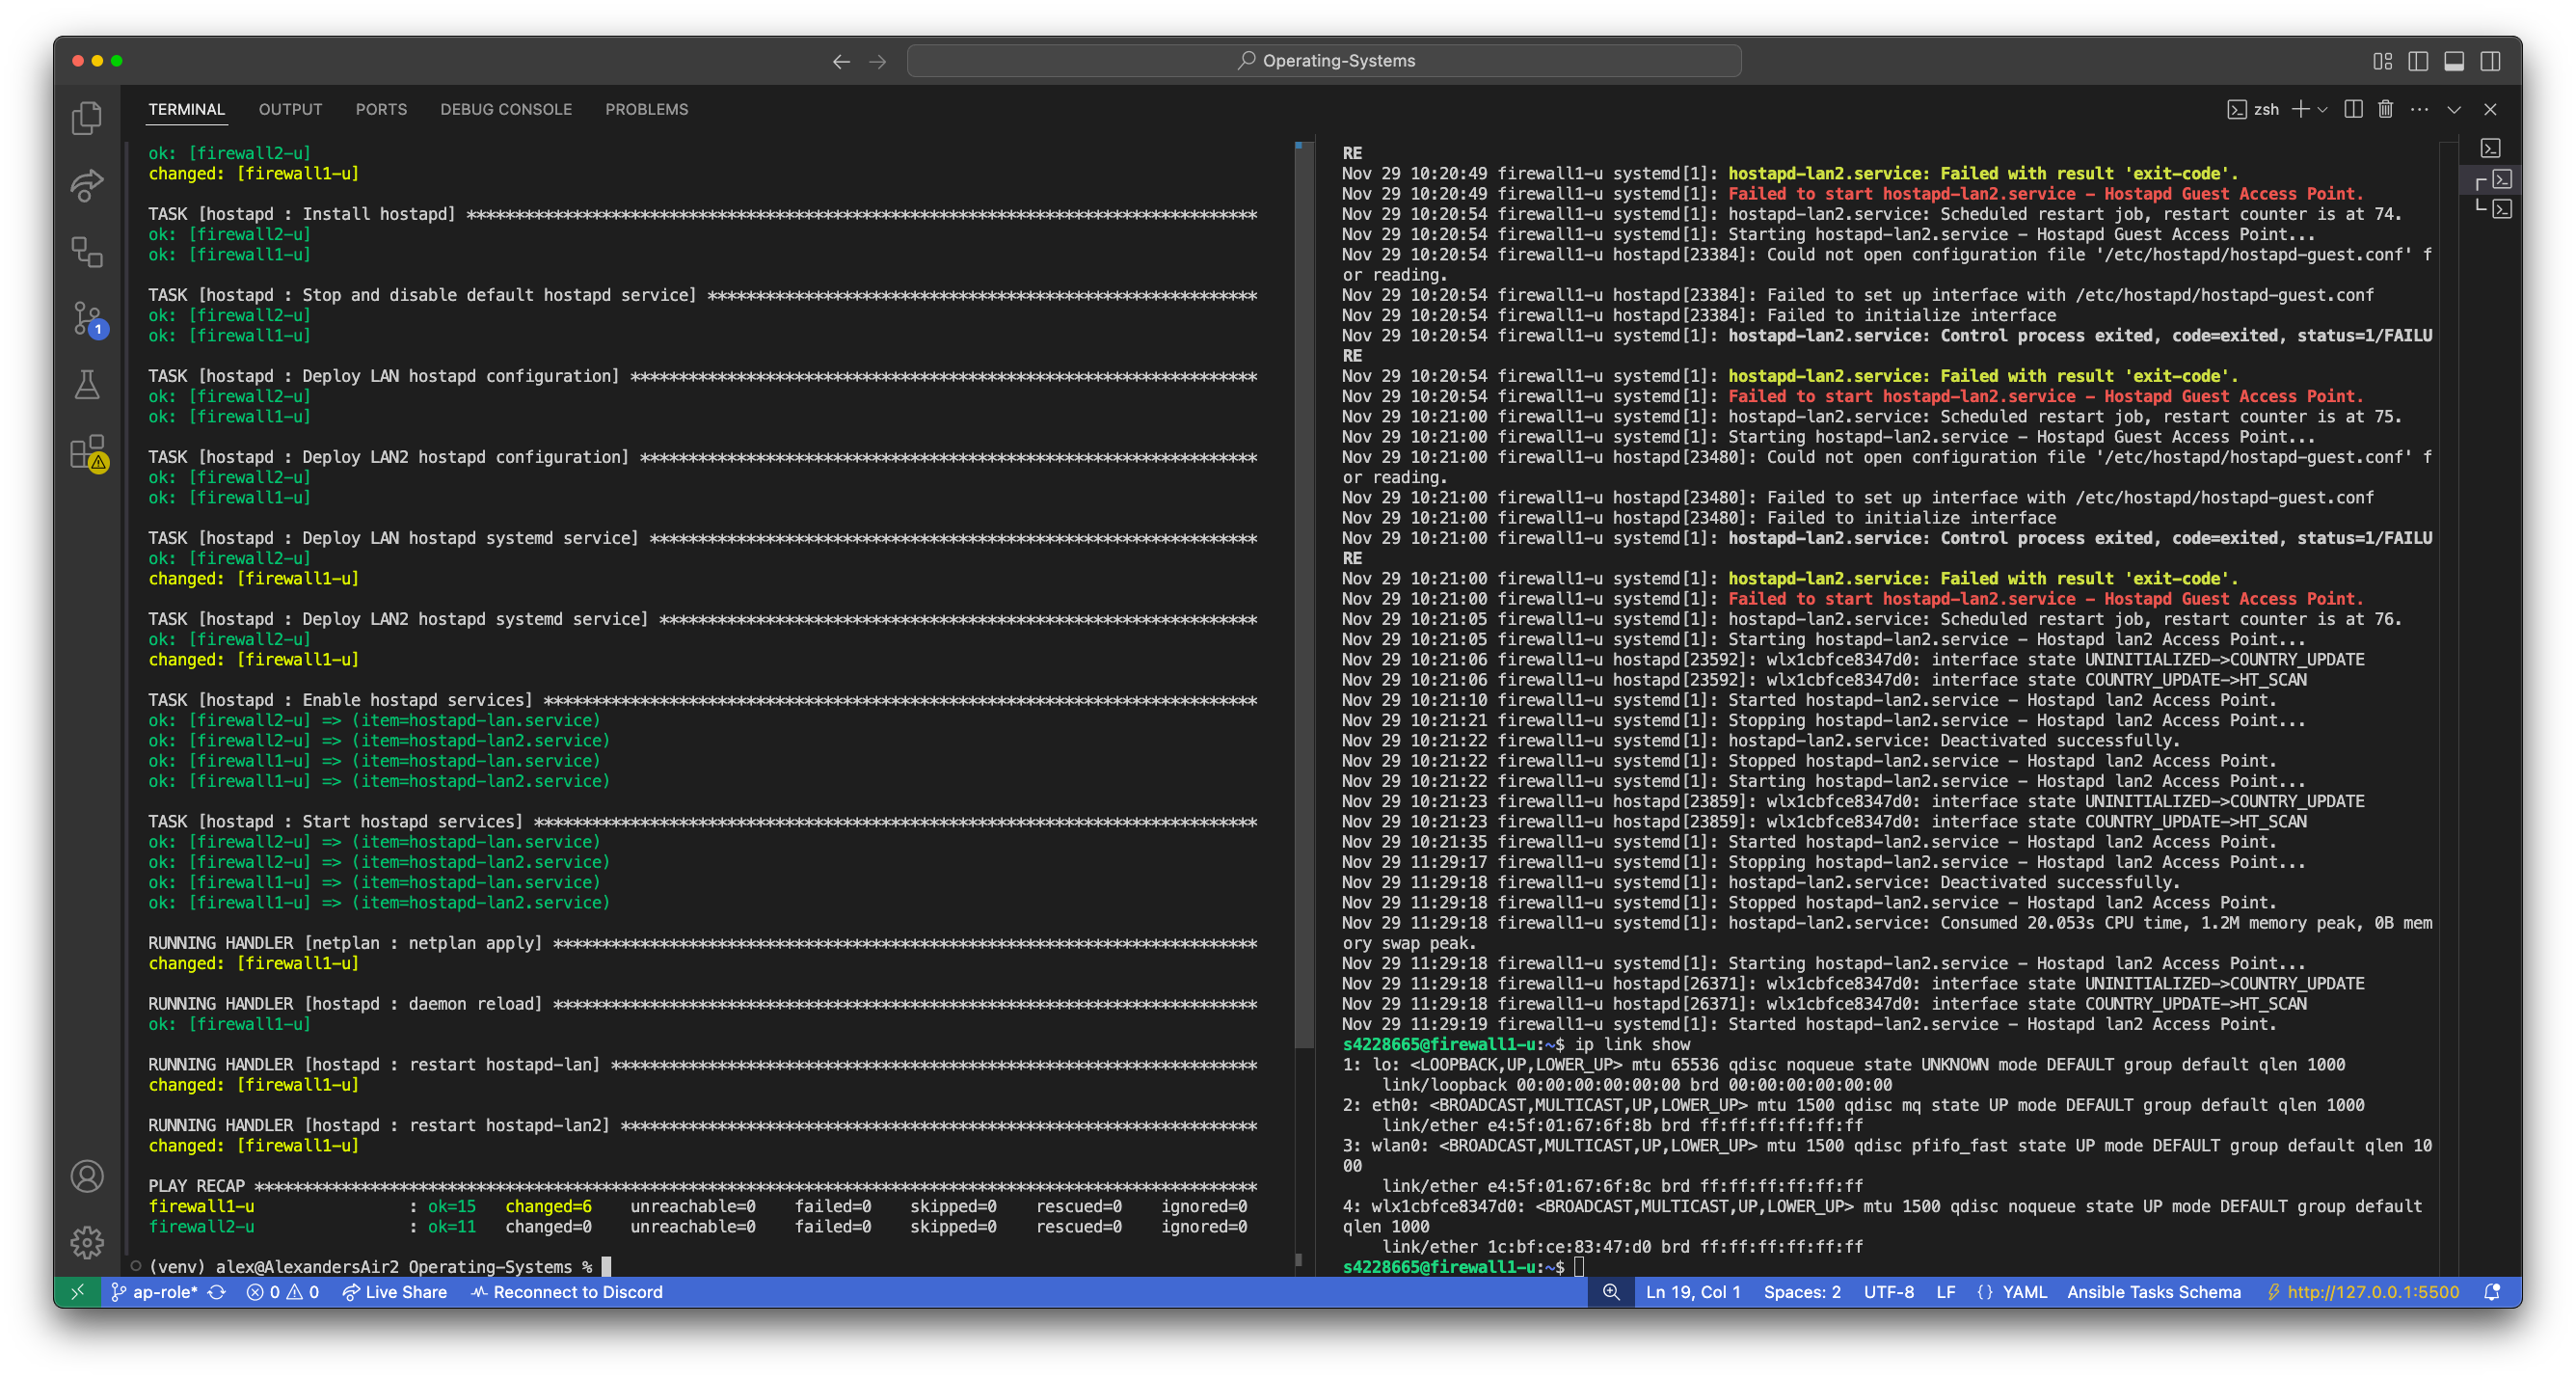
\includegraphics[width=1\linewidth]{Screenshots/vscode-both-firewall-deploy1.png}
    \caption{A successful firewall deployment on the LAN interface, but the LAN2 interface is still down}
    \label{fig:ansible-firewall-deploy1}
\end{figure}

After doing some troubleshooting (checking logs in figure \ref{fig:ansible-firewall-deploy1}) and seeing my own 2.4Ghz wifi go down, it looks like 

ISSUES









% Demo

The template uses Jinja2 variable substitution to separate configuration data from structure, enabling environment-specific deployments (testing vs. production) without modifying the template itself. Variables are defined in \texttt{roles/netplan/vars/main.yml} (Figure \ref{fig:netplan-vars}).

The WAN interface (\texttt{eth0}) is the only interface with a default route, ensuring all internet-bound traffic exits through the upstream gateway at \texttt{10.0.0.1}. The LAN and LAN2 interfaces (\texttt{eth1}, \texttt{eth2}) do not define routes, as the firewall itself is the gateway for these networks - routing decisions are handled by the iptables forwarding rules discussed in Section \ref{subsec:firewall-rules}.

DNS servers are configured only on the WAN interface using Google DNS (\texttt{8.8.8.8}) and Cloudflare DNS (\texttt{1.1.1.1}) as public resolvers. Internal zone devices receive DNS configuration via DHCP, which will be discussed in the DHCP server configuration (if implemented) or rely on the firewall to forward DNS queries.

\subsubsection{Configuration Verification}
\label{subsubsec:netplan-verify}

After Ansible deployment, the netplan configuration can be verified using the \texttt{ip addr} command to confirm all three interfaces have received their static IP addresses:

\begin{verbatim}
ubuntu@raspberrypi:~$ ip addr show
2: eth0: <BROADCAST,MULTICAST,UP,LOWER_UP> mtu 1500
    inet 10.0.0.2/8 brd 10.255.255.255 scope global eth0
3: eth1: <BROADCAST,MULTICAST,UP,LOWER_UP> mtu 1500
    inet 172.16.0.1/16 brd 172.16.255.255 scope global eth1
4: eth2: <BROADCAST,MULTICAST,UP,LOWER_UP> mtu 1500
    inet 192.168.0.1/24 brd 192.168.255.255 scope global eth2
\end{verbatim}

The \texttt{ip route} command confirms that the default route points to the WAN gateway, with directly connected routes for LAN and Guest subnets:

\begin{verbatim}
ubuntu@raspberrypi:~$ ip route show
default via 10.0.0.1 dev eth0 proto static
10.0.0.0/8 dev eth0 proto kernel scope link src 10.0.0.2
172.16.0.0/16 dev eth1 proto kernel scope link src 172.16.0.1
192.168.0.0/24 dev eth2 proto kernel scope link src 192.168.0.1
\end{verbatim}